% Template for Elsevier CRC journal article
% version 1.1 dated 16 March 2010

% This file (c) 2010 Elsevier Ltd.  Modifications may be freely made,
% provided the edited file is saved under a different name

% This file contains modifications for Procedia Computer Science
% but may easily be adapted to other journals

% Changes since version 1.0
% - elsarticle class option changed from 1p to 3p (to better reflect CRC layout)

%-----------------------------------------------------------------------------------

%% This template uses the elsarticle.cls document class and the extension package ecrc.sty
%% For full documentation on usage of elsarticle.cls, consult the documentation "elsdoc.pdf"
%% Further resources available at http://www.elsevier.com/latex

%-----------------------------------------------------------------------------------

%%%%%%%%%%%%%%%%%%%%%%%%%%%%%%%%%%%%%%%%%%%%%%
%%%%%%%%%%%%%%%%%%%%%%%%%%%%%%%%%%%%%%%%%%%%%%
%%                                          %%
%% Important note on usage                  %%
%% -----------------------                  %%
%% This file must be compiled with PDFLaTeX %%
%% Using standard LaTeX will not work!      %%
%%                                          %%
%%%%%%%%%%%%%%%%%%%%%%%%%%%%%%%%%%%%%%%%%%%%%%
%%%%%%%%%%%%%%%%%%%%%%%%%%%%%%%%%%%%%%%%%%%%%%

%% The '3p' and 'times' class options of elsarticle are used for Elsevier CRC
\documentclass[3p,times]{elsarticle}

%% The `ecrc' package must be called to make the CRC functionality available
\usepackage{ecrc}
%% The ecrc package defines commands needed for running heads and logos.
%% For running heads, you can set the journal name, the volume, the starting page and the authors

%% set the volume if you know. Otherwise `00'
\volume{00}

%% set the starting page if not 1
\firstpage{1}

%% Give the name of the journal
\journalname{Artificial Intelligence}

%% Give the author list to appear in the running head
%% Example \runauth{C.V. Radhakrishnan et al.}
\runauth{}

%% The choice of journal logo is determined by the \jid and \jnltitlelogo commands.
%% A user-supplied logo with the name <\jid>logo.pdf will be inserted if present.
%% e.g. if \jid{yspmi} the system will look for a file yspmilogo.pdf
%% Otherwise the content of \jnltitlelogo will be set between horizontal lines as a default logo

%% Give the abbreviation of the Journal.
\jid{procs}

%% Give a short journal name for the dummy logo (if needed)
\jnltitlelogo{Artificial Intelligence}

%% Hereafter the template follows `elsarticle'.
%% For more details see the existing template files elsarticle-template-harv.tex and elsarticle-template-num.tex.

%% Elsevier CRC generally uses a numbered reference style
%% For this, the conventions of elsarticle-template-num.tex should be followed (included below)
%% If using BibTeX, use the style file elsarticle-num.bst

%% End of ecrc-specific commands
%%%%%%%%%%%%%%%%%%%%%%%%%%%%%%%%%%%%%%%%%%%%%%%%%%%%%%%%%%%%%%%%%%%%%%%%%%

%% The amssymb package provides various useful mathematical symbols
\usepackage{amssymb}
%% The amsthm package provides extended theorem environments
%%\usepackage{amsthm}

%% The lineno packages adds line numbers. Start line numbering with
%% \begin{linenumbers}, end it with \end{linenumbers}. Or switch it on
%% for the whole article with \linenumbers after \end{frontmatter}.
%% \usepackage{lineno}

%% natbib.sty is loaded by default. However, natbib options can be
%% provided with \biboptions{...} command. Following options are
%% valid:

%%   round  -  round parentheses are used (default)
%%   square -  square brackets are used   [option]
%%   curly  -  curly braces are used      {option}
%%   angle  -  angle brackets are used    <option>
%%   semicolon  -  multiple citations separated by semi-colon
%%   colon  - same as semicolon, an earlier confusion
%%   comma  -  separated by comma
%%   numbers-  selects numerical citations
%%   super  -  numerical citations as superscripts
%%   sort   -  sorts multiple citations according to order in ref. list
%%   sort&compress   -  like sort, but also compresses numerical citations
%%   compress - compresses without sorting
%%
%% \biboptions{comma,round}

% \biboptions{}

% if you have landscape tables
\usepackage[figuresright]{rotating}

\usepackage{amsthm}
\usepackage{amsmath}
\usepackage{amssymb}
\usepackage{times}
\usepackage{helvet}
\usepackage{courier}
\usepackage{pstricks}
\usepackage{pst-node}
\usepackage{multirow}
\usepackage{listings}
\usepackage{xspace}


\usepackage{pgf}
\usepackage{tikz}
\usetikzlibrary{calc,backgrounds,positioning,fit}
\usepackage{subcaption}
\usetikzlibrary{arrows,automata}
\usepackage{arydshln}



% put your own definitions here:
%   \newcommand{\cZ}{\cal{Z}}
%   \newtheorem{def}{Definition}[section]
%   ...

\newtheorem{mytheorem}{Theorem}
\newtheorem{mylemma}[mytheorem]{Lemma}
\newtheorem{mydefinition}[mytheorem]{Definition}
\newtheorem{myconstruction}{Construction}


\mathchardef\mh="2D
\newcommand{\pre}{\mathsf{pre}}  % precondition
\newcommand{\eff}{\mathsf{eff}}  % effect
\newcommand{\cond}{\mathsf{cond}}   % conditional effect
\newcommand{\add}{\mathsf{add}}  % add effect
\newcommand{\del}{\mathsf{del}}  % delete effect
\newcommand{\PE}{\mathrm{PE}}     % precondition
\newcommand{\PSPACE}{\mathrm{PSPACE}}     % precondition
\newcommand{\NPSPACE}{\mathrm{NPSPACE}}     % precondition
\newcommand{\strips}{\textsc{Strips}}     % precondition


\newcommand{\ARMS}{{\small {\sffamily ARMS}}\xspace}
\newcommand{\CAMA}{{\small {\sffamily CAMA}}\xspace}
\newcommand{\SLAF}{{\small {\sffamily SLAF}}\xspace}
\newcommand{\LAMP}{{\small {\sffamily LAMP}}\xspace}
\newcommand{\NOISTA}{{\small {\sffamily NOISTA}}\xspace}
\newcommand{\LOCM}{{\small {\sffamily LOCM}}\xspace}
\newcommand{\LOCMtwo}{{\small {\sffamily LOCM2}}\xspace}
\newcommand{\LOP}{{\small {\sffamily LOP}}\xspace}
\newcommand{\AMAN}{{\small {\sffamily AMAN}}\xspace}
\newcommand{\FAMA}{{\small {\sffamily FAMA}}\xspace}

\newcommand{\FO}{{\small {\sffamily FO}}\xspace}
\newcommand{\PO}{{\small {\sffamily PO}}\xspace}
\newcommand{\POstar}{{\small {\sffamily PO*}}\xspace}
\newcommand{\NO}{{\small {\sffamily NO}}\xspace}

\newcommand{\pbox}[1]{\makebox[2em][l]{#1}}

\newcommand{\tup}[1]{{\langle #1 \rangle}}

\lstset{
  basicstyle=\ttfamily,
  mathescape
}

% add words to TeX's hyphenation exception list
%\hyphenation{author another created financial paper re-commend-ed Post-Script}

% declarations for front matter

\begin{document}

\begin{frontmatter}

%% Title, authors and addresses

%% use the tnoteref command within \title for footnotes;
%% use the tnotetext command for the associated footnote;
%% use the fnref command within \author or \address for footnotes;
%% use the fntext command for the associated footnote;
%% use the corref command within \author for corresponding author footnotes;
%% use the cortext command for the associated footnote;
%% use the ead command for the email address,
%% and the form \ead[url] for the home page:
%%
%% \title{Title\tnoteref{label1}}
%% \tnotetext[label1]{}
%% \author{Name\corref{cor1}\fnref{label2}}
%% \ead{email address}
%% \ead[url]{home page}
%% \fntext[label2]{}
%% \cortext[cor1]{}
%% \address{Address\fnref{label3}}
%% \fntext[label3]{}

\dochead{}
%% Use \dochead if there is an article header, e.g. \dochead{Short communication}

\title{Learning and Evaluation of \strips\ Action Models with Classical Planning}
\author[label1]{Diego Aineto}
\author[label1]{Sergio Jim\'{e}nez Celorrio}
\author[label1]{Eva Onaindia}
\address[label1]{Department of Computer Systems and Computation, Universitat Polit\`ecnica de Val\`encia. Spain}


%% use optional labels to link authors explicitly to addresses:
%% \author[label1,label2]{<author name>}
%% \address[label1]{<address>}
%% \address[label2]{<address>}


\begin{abstract}
  This paper presents a novel approach for learning \strips\ action models from observations of plan executions that compiles this learning task into classical planning. The compilation approach is flexible to various amount and kind of available input knowledge; learning examples can range from plans (with their corresponding initial state) to sequences of state observations or even just a set of initial and final states (where no intermediate action or state is known). The compilation accepts also partially specified action models and can be used to validate whether the observation of a plan execution follows a given \strips\ action model, even if this model is not fully specified. On the other hand, the compilation is extensible to assess how well a given \strips\ action model matches the observation of a plan execution. This extension allows us to evaluate the quality of the learned models with respect to the actual models but also, with respect to a {\em test set} of observations of plan executions. The performance of our compilation approach is evaluated learning action models, for a wide range of classical planning domains from the International Planning Competition (IPC), and following these two evaluation approaches.
\end{abstract}

\begin{keyword}
Classical planning\sep Learning action models\sep Generalized planning
%% keywords here, in the form: keyword \sep keyword

%% MSC codes here, in the form: \MSC code \sep code
%% or \MSC[2008] code \sep code (2000 is the default)
\end{keyword}

\end{frontmatter}

%%
%% Start line numbering here if you want
%%
% \linenumbers

%% main text

%% The Appendices part is started with the command \appendix;
%% appendix sections are then done as normal sections
%% \appendix

%% \section{}
%% \label{}

% HLP: Expressiveness is pushed when pure compilations are used. Otherwise we just use them.



\section{Introduction}
\label{sec:introduction}

Besides {\em plan synthesis}~\cite{ghallab2004automated}, planning action models are also useful for {\em plan/goal recognition}~\cite{ramirez2012plan}. At both planning tasks, automated planners reason about action models that correctly and completely capture the possible world transitions~\cite{geffner:book:2013}. Unfortunately, modeling planning actions is complex, even for planning experts, and this knowledge acquisition task is a bottleneck that limits the potential of AI planning~\cite{kambhampati:modellite:AAAI2007}.

Machine Learning (ML) has shown to be able to compute a wide range of different kinds of models from examples~\cite{michalski2013machine}. The application of inductive ML to the learning of \strips\ action models, the vanilla action model for automated planning~\cite{fikes1971strips}, is not straightforward though:
\begin{itemize}
\item The {\em input} to ML algorithms (the {\em learning/training} data) usually are finite vectors encoding the value of fixed features in a given set of objects. The input for learning planning action models are observations of plan executions (where each observed plan possibly has a different number of steps and involves a different number of objects).
\item The {\em output} of ML algorithms usually is a scalar value (an integer, in the case of {\em classification} tasks, or a real value, in the case of {\em regression} tasks). When learning \strips\ action models the output is, for each action, the sets of {\em preconditions}, {\em negative} and {\em positive effects} that define the possible state transitions.
\end{itemize}

Motivated by recent advances on the synthesis of different kinds of generative models with classical planning~\cite{bonet2009automatic,segovia2016generalized,segovia2016hierarchical,segovia2017generating}, this paper introduces an innovative approach for learning \strips\ action models that can be defined as a classical planning compilation. A solution to the classical planning task that results from our compilation is a sequence of actions that determines the preconditions and effects of a \strips\ model such that this model satisfies the plan executions given as input.

The compilation approach is appealing by itself because it leverages off-the-shelf planners and because its practicality allow us to report learning results over a wide range of domains from the {\em International Planning Competition} (IPC). Moreover, it opens up a way towards \emph{bootstrapping} planning action models, enabling a planner to gradually learn/update its action model. Apart from these, our compilation exhibits the following contributions:
\begin{enumerate}
\item {\bf\em Input flexibility}. Our classical planning compilation is flexible to various amount and kind of available input knowledge. The action model to learn can be partially specified and the learning examples can range from a set of plans (with their corresponding initial state) or state observations, to just a set of initial and final states where no intermediate action or state is observed. % Also accepts background knowledge

\item {\bf\em Model validation}. The compilation poses a novel framework to assess the validation of a STRIPS model with respect a plan execution. This validation capacity goes beyond the functionality of VAL~\cite{howey2004val} since it does require neither a full action model nor a fully observed plan to determine validation. 
  
\item {\bf\em Model evaluation}. The compilation can assess how well a given \strips\ action model matches a plan execution, which allows us to assess learning performance without having the actual action model. The idea is to assess the amount of edition that is required by the input action model to induce the given observation of the plan execution. 
\end{enumerate}

A first description of the compilation previously appeared in our conference paper~\cite{aineto2018learning}. Compared to that conference paper, this work includes the following novel material:
\begin{itemize}
\item A unified formulation for learning and evaluating \strips\ action models from observed executions of plans. Further, these executions can only comprise state observations.
\item A redefinition of the ML metrics {\em precision} and {\em recall} to evaluate \strips\ action models with respect to observations of plan executions.
%\item Leveraging diverse forms of {\em background knowledge} for learning and evaluating \strips\ action models.
\item A complete empirical evaluation of the compilation approach. Our evaluation analyses how the amount of input knowledge affects to the performance of the compilation approach when learning and evaluating \strips\ action models. 
\end{itemize}

Section~\ref{sec:background} introduces classical planning and reviews related work on learning planning action models. Section~\ref{sec:Section3} introduces the classical planning model and the \strips\ action model (the target of our learning and evaluation tasks). Section~\ref{sec:Section4} formalizes the learning of \strips\ action models with regard to different amount and kind of available input knowledge. Sections~\ref{sec:Section5} and ~\ref{sec:Section6} describe our compilation approach for addressing the formalized learning tasks its extension to evaluate and recognize \strips\ action models. Section~\ref{sec:Section7} reports the data collected in a two-fold empirical evaluation of our learning approach: First, the learned \strips\ action models are tested with observations of plan executions and second, the learned models are compared to the actual models. Finally, Section ~\ref{sec:Section8} discusses the strengths and weaknesses of the compilation approach and proposes several opportunities for future research.

 


\section{Background}
\label{sec:background}

This section serves two purposes; first, we introduce basic planning concepts and define the classical planning model we aim to learn; secondly, we summarize the most relevant existing approaches to learn classical planning action models.



\subsection{Basic planning concepts}
\label{basic_planning}


We use $F$ to denote the set of {\em fluents} (propositional variables) describing a state. A {\em literal} $l$ is a valuation of a fluent $f\in F$, i.e. either~$l=f$ or $l=\neg f$. A set of literals $L$ represents a partial assignment of values to fluents (without loss of generality, we will assume that $L$ does not assign conflicting values to any fluent). The complement of $L$ is defined as $\neg L=\{\neg l:l\in L\}$. We use $\mathcal{L}(F)$ to denote the set of all literal sets on $F$, i.e.~all partial assignments of values to fluents.

We will adopt the \emph{open world assumption}, that is, what is not known to be true in a state is unknown, to implicitly represent the unobserved literals of states. Consequently, states will explicitly include positive literals ($f$) and negative literals ($\neg f$) such that literals that are not in a state are unknown or unobserved. Hence, a {\em state} $s$ is a full assignment of values to fluents; i.e. $|s|=|F|$, so the size of the state space is $2^{|F|}$. Like in PDDL~\cite{fox2003pddl2}, we assume that fluents $F$ are instantiated from a set of {\em predicates} $\Psi$. Each predicate $p\in\Psi$ has an argument list of arity $ar(p)$. Given a set of {\em objects} $\Omega$, the set of fluents $F$ is induced by assigning objects in $\Omega$ to the arguments of predicates in $\Psi$; i.e.~$F=\{p(\omega):p\in\Psi,\omega\in\Omega^{ar(p)}\}$ such that $\Omega^k$ is the $k$-th Cartesian power of $\Omega$.

A {\em classical planning frame} is a tuple $\Phi=\tup{F,A}$, where $F$ is a set of fluents and $A$ is a set of actions. An action $a\in A$ has a set of preconditions $\pre(a)\in\mathcal{L}(F)$ and a set of effects $\eff(a)\in\mathcal{L}(F)$. An action $a\in A$ is applicable in a given state $s$ iff $pre(a)\subseteq s$, i.e.~if the literals $pre(a)$ hold in $s$. The result of executing an applicable action $a\in A$ in a state $s$ is a new state $\theta(s,a)=\{s\setminus \neg\eff(a)\cup\eff(a)\}$. Note that subtracting the complement of $\eff(a)$ from $s$ ensures that $\theta(s,a)$ remains a well-defined state with positive and negative literals. Then:

\begin{itemize}
\item $\eff^+(a)\in\mathcal{L}(F)$ is the {\em positive effects} of $a$, the subset of action effects that assert a positive literal in the state resulting after the application of $a$
\item $\eff^-(a)\in\mathcal{L}(F)$ is the {\em negative effects} of $a$, the subset of action effects that assert a negative literal in the state resulting after the application of $a$
\end{itemize}

Since we restrict our attention to \strips\ action models learning, we will assume the set of syntactic constraints imposed by \strips\ models, namely that $\eff^-(a)\subseteq \pre(a)$, $\eff^-(a)\cap \eff^+(a)=\emptyset$ and $\pre(a)\cap \eff^+(a)=\emptyset$. Additionally, actions $a\in A$ are instantiated from given action schemas, as in PDDL.


A {\em classical planning problem} is a tuple $P=\tup{F,A,I,G}$, where $I$ is an initial state and $G\in\mathcal{L}(F)$ is a goal condition. A {\em plan} for $P$ is an action sequence $\pi=\tup{a_1, \ldots, a_n}$ that induces the {\em state trajectory} $s=\tup{s_0, s_1, \ldots, s_n}$ such that $s_0=I$ and, for each {\small $1\leq i\leq n$}, $a_i$ is applicable in $s_{i-1}$ and generates the successor state $s_i=\theta(s_{i-1},a_i)$. The {\em plan length} is denoted with $|\pi|=n$ . A plan $\pi$ {\em solves} $P$ iff $G\subseteq s_n$, i.e.,~if the goal condition is satisfied at the last state reached after following the application of the plan $\pi$ in the initial state $I$. A solution plan for $P$ is {\em optimal} if it has minimum length.

In this work, the term \emph{plan trace} refers to the \emph{observation} of a plan execution that starts on a given initial state. A plan trace $\tau = \langle s_0, a_1, s_1, a_2, s_2, \ldots, a_n, s_n \rangle$ is generally defined as an interleaved combination of a sequence of executed actions $\tup{a_1, \ldots, a_n}$ and the induced state trajectory $\tup{s_0, s_1, \ldots, s_n}$. \emph{Plan traces} constitute the input knowledge of the learning tasks addressed in this paper.

Our approach copes with partial observability in the plan traces. Let $\pi=\tup{a_1, \ldots, a_n}$ be the plan executed by an agent that induces the state trajectory $s=\tup{s_0, s_1, \ldots, s_n}$, and let $\tau = \langle s_0, \ldots, a_i, \ldots, s_j, \ldots, s_n \rangle$ be the plan trace observed from the plan execution. With regards to the observed states of $\tau$, that we will refer to as $\tau_s$, we identify two general cases of observability:

\begin{enumerate}
\item we say that $\tau_s$ is a fully-observable (\FO) state trajectory if every observed intermediate state of $\tau_s$ is a full assignment of values to fluents, and there exists a single action that transitions from every state $s_i$ to state $s_{i+1}$ in $\tau_s$;  that is $\theta(s_i,\tup{a})=s_{i+1}$. This case clearly states that $\tau_s = s$, meaning that $\forall s_i \in \tau_s$, $s_i$ comprises all the literals of the corresponding state in the trajectory $s$ of the plan $\pi$. Formally, $\forall i, 1 \leq i  < n, |s_i| = |F|$.
\item we say that $\tau_s$ is a partially-observable (\PO) state trajectory if at least one intermediate state of $\tau_s$ is a partial assignment of values to fluents. Formally, $\exists i, 1 \leq i  < n, |s_i| < |F|$. This means that one or more literals are missing in the intermediate $s_i$, all of which may be missing. When all literals are missing, $s_i$ is a \emph{missing} or \emph{empty state} ($s_i = \emptyset$).
\end{enumerate}

The general definition of a \PO state trajectory gives rise to two special cases:

\begin{enumerate}
\item when \textbf{all} of the $n-1$ intermediate states of $s$ are \textbf{missing} in $\tau_s$, $\tau_s$ is a \emph{non-observable} (\NO) state trajectory. Formally, $\forall i, 1 \leq i < n,  s_i= \emptyset$; i.e., $|s_i| = 0$.
\item when \textbf{none} of the $n-1$ intermediate states of $s$ are \textbf{missing} in $\tau_s$, we will refer to $\tau_s$ as a \POstar state trajectory. Formally, $\exists i, 1 \leq i < n, s_i \neq \emptyset$; i.e., $0 < |s_i| < |F|$.
\end{enumerate}

Table \ref{tab:state_trajectory} summarizes the four types of state trajectories according to the observed information, which ultimately affects the number of observed intermediate states and the number of literals comprised in each intermediate state. \PO comprises both \POstar and \NO, and it thus encompasses trajectories with some missing state.

\begin{table}[hbt!]
\centering
\begin{tabular}{c|c|c|}
	     & {\bf \# intermediate states} & {\bf state type} \\ \hline
    \FO & $n-1$  & {\small $\forall i, 1 \leq i < n$}  \\  & & $s_i$ is a full assignment $|s_i|=|F|$ \\ \hline
    \multirow{1}{*}{\POstar} & $n-1$ & {\small $\exists i, 1 \leq i < n$}  \\ & & $s_i$ is a partial assignment $0 < |s_i|< |F|$\\ \hline
    \multirow{1}{*}{\PO} & $\leq n-1$ & {\small $\exists i, 1 \leq i < n$}   \\  & & $s_i$ is a partial assignment $|s_i|< |F|$\\ \hline
    \NO & 0 & {\small $\forall i, 1 \leq i < n$}  \\  & & $s_i$ is an empty state  $|s_i|=0$
\end{tabular}
\caption{Classification of state trajectories accordingly to the observed information.}
\label{tab:state_trajectory}
\end{table}


\FAMA can also deal with partial observability in the observed actions of $\tau$, that we will refer to as $\tau_a$. We identify three levels of observability, from the greatest to the lowest:

\begin{enumerate}
\item when \textbf{all} of the actions of $\pi$ appear in $\tau_a$, we say that $\tau_a$ is a fully-observable (\FO) action sequence; i.e.,  $\tau_a=\pi$. In this case, $\tau_a$ contains all the necessary actions to transit every state $s_{i-1}$ to its corresponding successor state $s_{i}$, from $s_0$ to $s_n$. This is the type of input trace accepted by all the existing learning approaches (see section \ref{related_work} for details).
\item when \textbf{some} of the actions of $\pi$  appear in $\tau_a$, we say that $\tau_a$ is a partially observable (\PO) action sequence. In this case, at least one of the necessary actions of the plan $\pi$ is missing in $\tau_a$. Formally, $\exists i, 1 \leq i \leq n, a_i \in \pi \wedge a_i \notin \tau_a$.
\item when \textbf{none} of the actions of $\pi$  appear in $\tau_a$, we say that $\tau_a$ is a non-observable (\NO) action sequence. Formally, $\forall i, 1 \leq i \leq n, a_i \in \pi \wedge a_i \notin \tau_a$. That is, $\tau_a = \emptyset$.
\end{enumerate}


Plan traces can be classified accordingly to the type of observed state trajectory (\FO, \POstar, \PO or \NO) and action sequence (\FO, \PO or \NO). In section \ref{task_definition}, we expose the impact of the combinations of observed state trajectories and observed action sequences when solving a learning task.



\subsection{Related work}
\label{related_work}

In this section we summarize the most recent and relevant approaches to learning action models found in the literature. Approaches will be examined according to the following parameters: the observability of the plan traces accepted by the system, the expressiveness of the learned action model and the principal technique used for learning the action model (Table \ref{table:models_comparison1}), as well as the characteristics of the evaluation method used to validate the learned models (Table \ref{table:models_comparison2}).

The first column of Table \ref{table:models_comparison1} shows the constraints imposed on the input plan traces with regard to observability. Since all approaches except ours deal only with \FO action sequences, constraints are exclusively concerned with the type of state trajectory. This directly affects the complexity of the task, which can be sorted from the least to the most constrained following this order: 1) \NO, 2) \PO, 3) \POstar, and 4) \FO. Note that \PO is less constrained than \POstar because \PO considers the possibility of having some missing state in the trajectory.

The task of learning from less constrained traces subsumes learning from more constrained ones. Consequently, approaches to learning from, say traces with \PO state trajectories, will also enable learning from traces with \POstar state trajectories. All the approaches analyzed in this work accept the more constrained definition of partial observations of intermediate states \POstar, two of them also allow the sequence of intermediate states to be empty (\PO) and the majority accept \NO state trajectories. Exceptionally, \LOCM is the only approach capable of learning from a fully-empty state trajectory, with neither initial nor final state.


The expressiveness of the learned action models varies across approaches (second column of Table \ref{table:models_comparison1}). All the presented systems are able to learn action models in a \textsc{Strips}  representation \cite{fikes1971strips} and some propose algorithms to learn more expressive action models that include quantifiers, logical implications or the type hierarchy of a PDDL domain.

Table \ref{table:models_comparison2} summarizes the main characteristics of the evaluation of the learned action models based on the type of evaluation method (first column of Table \ref{table:models_comparison2} -- almost all approaches rely on a comparison between the learned model and a {\em Ground-Truth Model}), the metrics used in the comparison (second column of Table \ref{table:models_comparison2}) and the number of tested domains alongside the size of the training dataset (third column of Table \ref{table:models_comparison2}).

In the following, we present a comprehensive insight of the particularities of the seven systems presented in Table \ref{table:models_comparison1} and Table \ref{table:models_comparison2}. This exposition will also help us to highlight in section \ref{task_definition} the value of our contribution \FAMA.


\vspace{0.3cm}

The Action-Relation Modeling System (\textbf{\ARMS})~\cite{yang2007learning} is one of the first learning algorithms able to learn from plan traces with partial or null observations of intermediate states. \ARMS uncovers a number of constraints from the plan traces in the training data that must hold for the plans to be correct. These constraints are then used to build and solve a weighted propositional satisfiability problem with a MAX-SAT solver. Three types of constraints are considered: 1) constraints imposed by general axioms of correct \textsc{Strips} actions, 2) constraints extracted from the distribution of actions in the plan traces and 3) constraints obtained from the \PO states, if available. Frequent subsets of actions in which to apply the two latter types of constraints are found by means of frequent set mining.

\ARMS defines an error metric and a redundancy metric to measure the correctness and conciseness of an action model over the test set of input plan traces using a cross-validation evaluation. The model evaluation is posed as an optimization task that returns the model that best explains the input traces by minimizing the error and redundancy functions. This yields a model that is approximately correct (100\% correctness is not required so as to ensure generality and avoid overfitting), approximately concise (low redundancy rates), and that can explain as many examples as possible. Hence, there is no guarantee that the learned model of \ARMS explains all observed plans, not even that it correctly explains any of the plan traces of the test set.

The \ARMS system became a benchmark in action-model learning, showing empirically that is is feasible lo learn a model in a reasonably efficient way using a weighted MAX-SAT even with \NO state trajectories.


\begin{table}
	\small
	\centering
	\begin{tabular}{ l | c | c | c }
		& \multicolumn{1}{c|}{\bf Input plan traces}
        & \multicolumn{1}{c|}{\bf Learned action model}
        & \multicolumn{1}{c}{\bf Technique}     \\
		\hline			
		\multirow{2}{*}{\ARMS} & \NO states & \strips & MAX-SAT \\ & \FO actions & & \\
        \hline
        \multirow{2}{*}{\SLAF} & \POstar states  & universal quantifiers in $\eff$ & logical inference \\ & \FO actions &  & SAT solver \\
         \hline
		\multirow{2}{*}{\LAMP} & \PO states &  quantifiers &  Markov logic networks \\  & \FO actions & logical implications &  \\
         \hline
         \AMAN & \NO states & \strips & graphical model estimation \\ & noisy actions & & \\
         \hline
         \NOISTA & \POstar and noisy states & \strips &  classification \\ & \FO actions & & \strips \texttt{} rules derivation \\
         \hline
         \CAMA & \PO states &  \strips & crowdsourcing annotation\\ & \FO actions &  & MAX-SAT \\
         \hline
         \LOUGA & \NO states & \strips & Genetic algorithm \\ & \FO actions & negative preconditions & \\
         \hline
         \LOCMtwo & --- &  predicates and types & Finite State Machines \\ & \FO actions & & \\
         \hline
		\FAMA & \NO states & \strips &   compilation to planning\\ & \NO actions & & \\
         \hline
	\end{tabular}
	\caption{Characteristics of action-model learning approaches}
	\label{table:models_comparison1}
\end{table}	

A tractable and exact solution of action models in partially observable domains using a technique known as Simultaneous Learning and Filtering (\textbf{\SLAF}) is presented in~\cite{AmirC08}. \SLAF alongside \ARMS can be considered another of the precursors of the modern algorithms for action-model learning, able to learn from partially observable states. Given a formula representing the initial belief state, a sequence of executed actions and the corresponding partially observed states, \SLAF builds a complete explanation of observations by models of actions through a CNF formula. The learning algorithm updates the formula of the belief state with every action and observation in the sequence such that the new transition belief formula represents all possible transition relations consistent with the actions and observations at every time step.

\SLAF extracts all satisfying models of the learned formula with a SAT solver. For doing so, the training data set for each domain is composed of randomly generated action-observation sequences  (1,000 randomly selected actions and 10 fluents uniformly selected at random per observation). Additional processing in the form of replacement procedures or extra axioms are run into the SAT solver when finding the satisfying models. The experimentally tested \SLAF version is an algorithm that learns only effects for actions that have no conditional effects and assumes that actions in the sequences are all executed successfully (without failures). This algorithm cannot effectively learn the unknown preconditions of the actions and in the resulting models `\emph{one can see that the learned preconditions are often inaccurate}` \cite{AmirC08}. On the other hand, it does not report any statistical evaluation of measurement error other than a manually comparison of the learned models with a ground-truth model.

The Learning Action Models from Plan Traces (\textbf{\LAMP}) \cite{ZhuoYHL10} algorithm extends the expressiveness to learning models with universal and existential quantifiers as well as logical implications. The input to \LAMP is a set of plan traces with intermediate states, which are encoded by the algorithm into propositional formulas. \LAMP then uses the action headers and predicates to build a set of candidate formulas that are validated against the input set using a Markov Logic Network and effectively weighting each formula. The formulas with weights larger than a certain threshold are chosen to represent preconditions and effects of the learned action models.

\LAMP allows \PO state trajectories up to a minimum observability of 1/5 of non-empty states as well as \POstar state trajectories with different degrees of observability in the number of propositions in each state. It uses an error metric based on counting the differences in the number of precondition and effects between the ground-truth model and the learned model. In general, the results show that the accuracy of the learned models is fairly sensitive to the threshold chosen to learn the weights of the candidate formulas, and that domains that feature more conditional effects are harder to learn.


\begin{table}
	\small
	\centering
	\begin{tabular}{ l | c | c | c }
		%& \multicolumn{1}{c}{Evaluation task}
        & \textbf{Evaluation method} & \textbf{Metrics} & \textbf{\#tested domains/}   \\
        &   &   & \textbf{training data size} \\
		\hline			
		\multirow{1}{*}{\ARMS} & cross-validation with a test set & error counting of \#$\pre$ satisfaction  & 6  \\
        & of plan traces & and redundancy & 1,600-4,320 actions\\ & & & (160 plan traces) \\
        \hline
         \SLAF &  manual checking wrt GTM &  ---   & 4\\ & & & 1,000 actions\\
         \hline
		\multirow{1}{*}{\LAMP} & checking wrt GTM  & error counting of extra & 4\\ & & and missing \#$\pre$ and \#$\eff$ & 1,300-6,100 actions\\
           & & & (100-200 plan traces) \\
         \hline
         \AMAN & checking wrt GTM &  error counting of extra &  3 \\ & & and missing \#$\pre$ and \#$\eff$ & 40-200 plan traces\\
         \hline
         \NOISTA & checking wrt GTM  & error counting of extra & 5\\ & & and missing \#$\pre$ and \#$\eff$ & 5,000-20,000 actions\\
         \hline
         \CAMA & checking wrt GTM  &  error counting of extra & 3 \\ & & and missing \#$\pre$ and \#$\eff$ & 15-75 plan traces\\
         \hline
       \LOUGA & cross-validation with & redundant effects & 5 \\  & a test set of plan traces & differences wrt the test set & 800 - 3200 actions (160 traces)\\
         \hline
		\LOCMtwo & manual checking wrt GTM &  ---  &   --- \\
         \hline
		\FAMA & checking wrt GTM  & precision and recall & 15\\  & validation with a test set &  & 20-50 actions\\
         \hline
	\end{tabular}
	\caption{Evaluation of action models (GTM: ground-truth model)}
	\label{table:models_comparison2}
\end{table}	


The Action Model Acquisition from Noisy plan traces (\textbf{\AMAN}) \cite{zhuo2013action} introduces an algorithm able to learn action models from plan traces with \NO state sequences where actions have a probability of being observed incorrectly (noisy actions). The first step of the \AMAN algorithm is to build the set of candidate domain models that are consistent with the action headers and predicates. \AMAN then builds a graphical model to capture the domain physics; i.e., the relations between states, correct actions, observed actions and domain models. After that, the parameters of the graphical model are learned, computing at the same time the probability distribution of each candidate domain model. \AMAN finally returns the model that maximizes a reward function defined in terms of the percentage of actions successfully executed and the percentage of goal propositions achieved after the last successfully executed action.

\AMAN uses the same metric as \LAMP, namely counting the number of preconditions and effects that appear in the learned model and not in the ground-truth model (extra fluents) and viceversa (missing fluents). In a comparison between \AMAN and \ARMS on noiseless inputs, the results show that the accuracy of the learnt models are very close to each other and neither dominates the other. The convergence property of \AMAN guarantees that the accuracy of the learned model with noisy input traces becomes more and more close to the case  \emph{without noise} because the distribution of noise in the plan becomes gradually closer to real distribution with the number of iterations.


Another interesting approach that deals with noisy and incomplete observations of states is presented in \cite{MouraoZPS12}. We will refer to this approach as \textbf{\NOISTA} henceforth. In \NOISTA, actions are correctly observed but they can obviously be unsuccessfully executed in the possibly noisy application state. The basis of this approach consists of two parts: a) the application of a voted Perceptron classification method to predict the effects of the actions in vectorized state descriptions and b) the derivation of explicit \strips \texttt{} action rules to predict each fluent in isolation. Experimentally, the error rates in \NOISTA fall below 0.1 after 5,000 training samples for the five tested domains under a maximum of 5\% noise and a minimum of 10\% of observed fluents.

The Crowdsourced Action-Model Acquisition (\textbf{\CAMA}) \cite{Zhuo15} explores knowledge from both crowdsourcing (human annotators) and plan traces to learn action models for planning. \CAMA relies on the assumption that obtaining enough training samples is often difficult and costly because there is usually a limited number of plan traces available. In order to overcome this limitation, \CAMA builds on a set of soft constraints based on labels \texttt{true} or \texttt{false} given by the crowd and a set of soft constraints based on the input plan traces. Then it solves the constraint-based problem using a MAX-SAT solver and converts the solution to action models.

Plan traces in \CAMA are composed of 80\% of empty states and each partial state was selected by 50\% of propositions in the corresponding full state. An experimental comparison reveals that a manual crowdsourcing of \CAMA outperforms \ARMS and that as expected the difference becomes smaller as the number of plan traces becomes larger. The accuracy of \CAMA for a small number of plan traces (e.g., 30) is not less than 80\%, thus revealing that exploiting the knowledge of the crowd can help learning action models.


One of the latest incorporations to the family of action model learning algorithms is \LOUGA. This system uses a genetic algorithm to learn the effects of actions. In order to do this, each gene in the genome encodes whether a predicate is a positive effect, negative effect or none for a particular action, and the fitness of an individual is evaluated by reproducing the trace with the model encoded in the individual. After a solution for the effects is found, an ad-hoc algorithm is used to infer preconditions by finding those literals that are always present before the execution of an action. \LOUGA evaluates the learned models via cross-validation using the same metrics they use in their fitness function. In more detail, they measure (1) redundant positive and negative effects, (2) preconditions not met, and (3) literals observed in the input trace but not in the corresponding execution of the plan with the learned model.

\vspace{0.15cm}


Finally, we present the Learning Object-Centred Models (\textbf{\LOCM}), possibly the most distinctive learning system due to its ability of learning with minimal input knowledge. \textbf{\LOCM} only requires the \FO action sequence of the plan trace, without need for providing any information about the predicates or the state trajectory, not even the initial or final state~\cite{CresswellMW09,cresswell2013acquiring}. The lack of available state information is overcome by exploiting assumptions about the structure of the actions. Particularly, \LOCM assumes that objects found in the same position in the header of actions are grouped as a collection of objects named \emph{sort} whose defined set of states is captured by a parameterized Finite State Machine (FSM). The intuitive assumptions of \LOCM, like the continuity of object transitions or the association of parameters between consecutive actions in the training dataset, yield a learning model heavily reliant on the kind of domain structure. A later work, \textbf{\LOCMtwo}, extends the applicability of the \LOCM algorithm to a wider range of domains by introducing a richer representation that allows using multiple FSMs to represent the state of a \emph{sort}~\cite{cresswell2011generalised}.

\LOCMtwo is not experimentally evaluated, only the outcome of running the \LOCMtwo algorithm on several benchmark domains wrt to the reference model is reported in ~\cite{cresswell2011generalised}. It is worth noting the last contribution of the \LOCM family, called \textbf{\LOP} (\LOCM with Optimized Plans), addresses the problem of inducing static predicates~\cite{GregoryC16}. \LOP applies a post-processing step after the \LOCM analysis and it requires additional input information, particularly a set of optimal plans besides the suboptimal \FO action sequences.

The distinctive feature of the \LOCM family lies in the capacity to learn the state variables (fluents) because predicates are neither provided as input nor they are deducible from the plan trace as no state observability is allowed. In contrast, \FAMA and the rest of approaches either assume the set of predicates are provided alongside the input traces or assume they are extractable from the observed states of the plan trace, in which case the plan trace must comprise at least a grounded sample of every predicate. Similarly, the syntax of an action header (the action name and its parameters) is either extractable from the action sequence of the plan trace or it must be explicitly provided.








\section{Motivation}
\label{sec:motivation}

The main novelty of \FAMA with respect to other approaches lies in that our system is capable of handling \PO and \NO action sequences, which combined with \PO and \NO state trajectories, make the learning task more challenging. This essentially brings one key difference: the transition between two given observed states may now involve more than one action; i.e., $\theta(s_i,\tup{a_1,\ldots,a_k})=s_{i+1}$, with $k \geq 1$, $k$ unknown and unbound, and so the horizon of the input plan traces is no longer known now.

In this particular scenario, the actual number of plan traces that can correspond with the given input observations is also unbound and grows exponentially with the actual length of the plan trace (that is now unknown). Otherwise, the learning task is SAT compilable, which is known to be a NP-complete task~\cite{russell2016artificial}. This is the reason that SAT solving is a common technique in the approaches presented in section \ref{sec:background}.

When we assume partial observability in both the sequence of actions and the state trajectory, a complete approach must consider the length of the input plan traces to be unknown. This work shows that classical planning is a complete approach for this particular scenario. Consequently, the new learning scenario features PSPACE-complete instead of NP-complete tasks, which motivates and justifies the use of planning techniques, as our proposal of compiling the learning task to a planning problem.

When the plan trace is fully observed, learning \strips\ action models is straightforward~\cite{jimenez2012review}. In this case the {\em pre-} and {\em post-states} of every action are available so action {\em effects} are derived lifting the literals that change between the pre and post-state of the corresponding action executions. Likewise {\em preconditions} are derived lifting the minimal set of literals that appears in all the pre-states of the corresponding action.


%In \FAMA we set a probability threshold of observability to each fluent and action, which determines the percentage of literals in each state and in turn the percentage of observed states (when the probability of every fluent is above the threshold, the result is a missing state). This way, \FAMA must always work under the assumption that the number and length of the input plan traces are unknown and so the task of learning an action model becomes as hard as solving a \strips planning problem. Consequently, the new learning scenario features PSPACE-complete instead of NP-complete tasks, which motivates and justifies the use of planning techniques, as our proposal of compiling the learning task to a planning problem.

%Thereby, solving this type of learning tasks justifies the use of techniques other than SAT solvers, as our proposal of compiling the learning task to a planning problem.


\begin{table}[ht]
\centering
\begin{tabular}{c|c|c|c|c|}
	& \multicolumn{4}{c|}{\emph{state observability}} \\ \cline{2-5}
	\multirow{1}{*}{\emph{action}} & \FO & \POstar & \PO & \NO\\ {\emph{observability}} & & & & \\ \hline
	\FO & - & NP-complete & NP-complete & NP-complete \\ \hline
	\PO & NP-complete & NP-complete & \textbf{PSPACE-complete} & \textbf{PSPACE-complete} \\ \hline
	\NO & NP-complete & NP-complete & \textbf{PSPACE-complete} & \textbf{PSPACE-complete} \\ \hline
\end{tabular}
\caption{Complexity of learning tasks according to the type of input trace}
\label{tab:complex}
\end{table}


Table \ref{tab:complex} displays the complexity of the learning task according to the type of input trace. The PSPACE-complexity happens when the length of the plan trace is a priori unbound, which results from the combination of the following two causes:

\begin{enumerate}
\item As many of the approaches in section \ref{sec:background} assume, there may be an unknown number of missing intermediate states in the trace because of partial state observability (\PO and \NO). The assumption of having \FO state trajectory means that the sensors are able to capture every state change at every instant which typically is unrealistic. Normally the process of getting state feedback from sensors (or the processing of the sensor readings) is associated with a given sampling frequency that misses intermediate data between two sensor readings.

\item There may be also an unbound number of missing actions in the plan trace because of partial observability. The common assumption of having \FO action sequences in a learning task is unrealistic in many domains because it implies the existence of human observers that annotate the observed action sequences. In some real-world applications, the observed and collected data are sensory data (e.g., home automation, robotics) or images (e.g. traffic) and one cannot rely on human intervention for labeling actions. Actually, learning the executed actions can also be part of the action-model learning task. Learning from unstructured data involves some prior processing to transform the sensor or image information into a predicate-like format before applying the action-model learning approach~\cite{AsaiF18}, and it also requires the ability of identifying action symbols. In this sense, \FAMA represents a step ahead towards learning action models without assuming observed actions.
\end{enumerate}


Regarding the evaluation of the learned action models, we can observe in Table \ref{table:models_comparison2} that most of the approaches use a similar syntactic metric that consists in (1) counting the missing and extra fluents that appear in the learned model wrt the GTM and (2), normalizing this error by the the total number of all the possible preconditions and effects of an action model. This is an \emph{optimistic} metric since error rates are not normalized by the size of the actual GTM model. Hence, because the set of preconditions and effects of the GTM model is usually smaller than the set of all possible preconditions and effects, it turns out the metric may output error rates below 100\% for totally wrong learned models. To overcome this limitation we propose to use two standard metrics from ML, {\em precision} and {\em recall}. These two metrics are frequently used in pattern recognition, information retrieval and binary classification and are more informative that simply counting the number of errors in the learned model or computing the {\em symmetric difference} between the learned and the reference model~\cite{davis2006relationship}.

The ARMS systems implement semantic metrics for evaluating the learned action models with respect to observations of plan executions that act as a {\em test set}. This semantic evaluation approach is suitable for scenarios where the GTM is not available, e.g. the traditional ML setting. For this scenario we propose semantic versions of the {\em precision} and {\em recall} that provide a notion of the soundness and completeness of the learned models with respect to input plan traces. Unlike the metrics defined by ARMS, our new semantic metrics do not accumulate errors caused by the same flaw in the learned model. 

A striking figure of Table \ref{table:models_comparison2} that emphasizes a relevant feature of \FAMA is the small size of the training dataset it requires in comparison to other approaches. Unlike extensive-data ML approaches, our work explores an alternative research direction to learn sound models from small amounts of plan traces. This is an important advantage, particularly in domains in which it is costly or impossible to obtain a significant number of training samples. Unlike \CAMA, our approach does not require human intervention to label samples as it is able to learn from very small datasets.

Finally, we would also like to point out that, as shown in section \ref{sec:experiments}, \FAMA is exhaustively evaluated over a wide range of domains (15 domains compared to the scarce number of tested domains of the rest of the approaches in Table \ref{table:models_comparison2}) and uses exclusively an \emph{off-the shelf} classical planner so it can benefit straightforward from the last advances in classical planning.





























\section{Learning task}
\label{sec:learning}
Here we formalize the \strips\ action model and the task of learning \strips\ action models from observations of plan executions.


\subsection{\strips\ action schemas}
This work addresses the learning and evaluation of PDDL action schemas that follow the \strips\ requirement~\cite{mcdermott1998pddl,fox2003pddl2}. Figure~\ref{fig:stack} shows the {\em stack} action schema, coded in PDDL, from a four-operator {\em blocksworld}~\cite{slaney2001blocks}.

\begin{figure}[hbt!]
\begin{footnotesize}
\begin{verbatim}
(:action stack
 :parameters (?v1 ?v2 - object)
 :precondition (and (holding ?v1) (clear ?v2))
 :effect (and (not (holding ?v1)) (not (clear ?v2)) (handempty) (clear ?v1) (on ?v1 ?v2)))
\end{verbatim}
\end{footnotesize}
 \caption{\small \strips\ operator schema coding, in PDDL, the {\em stack} action from a four-operator {\em blocksworld}.}
\label{fig:stack}
\end{figure}

To formalize the target of the learning and evaluation tasks, we assume that fluents $F$ are instantiated from a set of {\em predicates} $\Psi$, as in PDDL. Each predicate $p\in\Psi$ has an argument list of arity $ar(p)$. Given a set of {\em objects} $\Omega$, the set of fluents $F$ is induced by assigning objects in $\Omega$ to the arguments of predicates in $\Psi$, i.e.~$F=\{p(\omega):p\in\Psi,\omega\in\Omega^{ar(p)}\}$ s.t. $\Omega^k$ is the $k$-th Cartesian power of $\Omega$.

Let $\Omega_v=\{v_i\}_{i=1}^{\operatorname*{max}_{a\in A} ar(a)}$ be a new set of objects ($\Omega\cap\Omega_v=\emptyset$), denoted as {\em variable names}, and that is bound by the maximum arity of an action in a given planning frame. For instance, in a three-block {\em blocksworld} $\Omega=\{block_1, block_2, block_3\}$ while $\Omega_v=\{v_1, v_2\}$ because the operators with the maximum arity, {\small\tt stack} and {\small\tt unstack}, have arity two.

We define $F_v$, a new set of fluents s.t. $F\cap F_v=\emptyset$, produced instantiating $\Psi$ using only {\em variable names}, and that defines the elements that can appear in the action schemes. In {\em blocksworld} this set contains 11 elements, $F_v$={\small\tt\{handempty, holding($v_1$), holding($v_2$), clear($v_1$), clear($v_2$), ontable($v_1$), ontable($v_2$), on($v_1,v_1$), on($v_1,v_2$), on($v_2,v_1$), on($v_2,v_2$)\}}.

In more detail, for a given operator schema $\xi$, we define $F_v(\xi)\subseteq F_v$ as the subset of elements that can appear in that action schema. For instance, for the {\em stack} action schema $F_v({\tt stack})=F_v$ while $F_v({\tt pickup})$={\small\tt\{handempty, holding($v_1$), clear($v_1$), ontable($v_1$), on($v_1,v_1$)\}} excludes the elements from $F_v$ that involve $v_2$ because {\small\tt pickup($v_1$)} has arity one.

We assume also that actions $a\in A$ are instantiated from \strips\ operator schemas $\xi=\tup{head(\xi),pre(\xi),add(\xi),del(\xi)}$ where:
\begin{itemize}
\item $head(\xi)=\tup{name(\xi),pars(\xi)}$, is the operator {\em header} defined by its name and the corresponding {\em variable names}, $pars(\xi)=\{v_i\}_{i=1}^{ar(\xi)}$. The headers of a four-operator {\em blocksworld} are {\small\tt pickup($v_1$), putdown($v_1$), stack($v_1,v_2$)} and {\small\tt unstack($v_1,v_2$)}.
\item The preconditions $pre(\xi)\subseteq F_v$, the negative effects $del(\xi)\subseteq F_v$, and the positive effects $add(\xi)\subseteq F_v$ such that, $del(\xi)\subseteq pre(\xi)$, $del(\xi)\cap add(\xi)=\emptyset$ and $pre(\xi)\cap add(\xi)=\emptyset$.
\end{itemize}
Given the set of predicates $\Psi$ and the header of the operator schema $\xi$, $2^{2|F_v(\xi)|}$ defines the size of the space of possible \strips\ models for that operator. Note that the previous constraints require that negative effects appear as preconditions and that they cannot be positive effects and also, that a positive effect cannot appear as a precondition. For the {\em blocksworld}, $2^{2|F_v(stack)|}=4194304$ while for the {\tt pickup} operator this number is only 1024.

We say that two \strips\ operator schemes $\xi$ and $\xi'$ are {\em comparable} if both schemas have the same parameters so they share the same space of possible \strips\ models (formally, iff $pars(\xi)=pars(\xi'$). For instance, we can claim that blocksworld operators {\tt stack} and {\tt unstack} are {\em comparable} while  {\tt stack} and {\tt pickup} are not. Last but not least, two \strips\ action models $\mathcal{M}$ and $\mathcal{M}'$ are {\em comparable} iff there exists a bijective function $\mathcal{M} \mapsto \mathcal{M}^*$ that maps every $\xi\in\mathcal{M}$ to a comparable action schema $\xi'\in\mathcal{M'}$ and vice versa.


\subsection{Learning \strips\ action schemas from plan executions}
The {\em learning task} addressed in this paper corresponds to learning an action model by observing an agent(s) acting in the world. This learning task is formalized as a tuple $\Lambda=\tup{\mathcal{M},\Psi,\mathcal{T}}$:
\begin{itemize}
\item $\mathcal{M}$ is the set of {\em initial} operator schemas ({\em empty} or {\em partially specified} if some preconditions or effects are known) that define the actions of a given planning frame.
\item $\Psi$ is the set of predicates that define the abstract state space of that planning frame. 
\item $\mathcal{T}=\tup{s_0,a,_1,s_1,\ldots,a_n,s_{n}}$ is a plan trace that contains the sequence of {\em state observations} obtained watching the execution of a plan $\pi=\tup{a_1, \ldots, a_n}$. 
\end{itemize}

A {\em solution} to a $\Lambda=\tup{\mathcal{M},\Psi,\mathcal{T}}$ learning task is a set of operator schema $\mathcal{M}'$ that is compliant with the input model $\mathcal{M}$, the predicates $\Psi$, and the observed plan trace $\mathcal{T}$. Note that $\mathcal{M}$ can be inferred from $\mathcal{T}$ provided that the actions in $\mathcal{T}$ are {\em diverse} enough. Meaning that $\mathcal{T}$ contains at least one instantiation of every action scheme in $\mathcal{M}$. Likewise $\Psi$ can be inferred from $\mathcal{T}$ when at least the observation of a state $s\in \mathcal{T}$ is a full state, that is $|s|=|F|$.



In this paper we address the $\Lambda=\tup{\mathcal{M},\Psi,\mathcal{T}}$ learning task with the following assumptions:
\begin{enumerate}
\item Each input action scheme $\xi\in\mathcal{M}$ is at least composed of its $head(\xi)$,
\item The initial state $s_0\in\mathcal{T}$ is {\em fully observable}.
\item Intermediate actions $a_i\in\mathcal{T}$ and states $s_i\in\mathcal{T}$ s.t. {\small $1\leq i\leq n$}, can be {\em partially observable} (some fluents in $s_i$ are missing because it is unknown whether their value is either positive or negative). In the extreme, all actions $a_i$, {\small $1\leq i\leq n$}, can be missing (unobserved) provided that the final state $s_n$ is at least, partially observed. Likewise, all states $s_i$, {\small $1\leq i\leq n$}, can be missing (unobserved) provided that at least actions $a_i$, {\small $1\leq i\leq n$}, are partially observed.
 \item Observations in $\mathcal{T}$ are {\em noiseless}, meaning that if a fluent or an action is observed it is the correct value. 
\end{enumerate}
Figure~\ref{fig:example-plans} shows an example of a learning task $\Lambda=\tup{\mathcal{M},\Psi,\mathcal{T}}$, that corresponds to observing the execution of a four-action plan $\pi=\tup{\small\tt (unstack\ B\ A), (putdown\ B), (pickup\ A), (stack\ A\ B)}$ for inverting a two-block tower. In this example $\mathcal{T}=\langle s_0,${\small\tt (unstack\ B\ A), (putdown\ B), (pickup\ A), (stack\ A\ B)}$,s_4\rangle$ which means that only the first and last states are observed and the three intermediate states $s_1$, $s_2$ and $s_3$ are fully unknown. 

\begin{figure}[hbt!]
{\footnotesize\tt ;;;;;; Action headers in $\mathcal{M}$}  
\begin{footnotesize}  
\begin{verbatim}
(pickup ?v1) (putdown ?v1) (stack ?v1 ?v2} (unstack ?v1 ?v2)
\end{verbatim}
\end{footnotesize}
\vspace{0.2cm}
{\footnotesize\tt ;;;;;; Predicates $\Psi$}
\begin{footnotesize}
\begin{verbatim}
(handempty) (holding ?v1) (clear ?v1) (ontable ?v1) (on ?v1 ?v2)
\end{verbatim}
\end{footnotesize}
\vspace{0.2cm}
{\footnotesize\tt ;;;;;; Plan trace $\mathcal{T}$}
\begin{footnotesize}
\begin{verbatim}
;;; state observation #0
(clear B) (on B A) (ontable A) (handempty)
\end{verbatim}
\end{footnotesize}

\begin{footnotesize}
{\footnotesize\tt ;;; Plan $\pi$}
\begin{verbatim}
0: (unstack B A)
1: (putdown B)
2: (pickup A)
3: (stack A B)
\end{verbatim}
\end{footnotesize}

\begin{footnotesize}
\begin{verbatim}
;;; state observation #4
(clear A) (on A B) (ontable B) (handempty)
\end{verbatim}
\end{footnotesize}

 \caption{\small Task $\Lambda=\tup{\mathcal{M},\Psi,\mathcal{T}}$ for learning a {\em blocksworld} \strips\ action model from a four-action plan and two state observations.}
\label{fig:example-plans}
\end{figure}

The definition of the $\Lambda=\tup{\mathcal{M},\Psi,\mathcal{T}}$ learning task is also extensible to the more general case where the execution of $\tau$ plans is observed. In this case, $\mathcal{T}=\{t_1,\ldots,t_{\tau}\}$ where each $t\in \mathcal{T}$ is a plan trace $t=\tup{s_0^t,a,_1^t,s_1^t,\ldots,a_n^t,s_{n}^t}$ that satisfies the previous [2-4] assumptions.



\section{Compilation}
\label{sec:compilation}

Our approach for addressing a $\Lambda$ learning task is compiling it into a classical planning task with conditional effects. The intuition behind the compilation is that a solution to the resulting classical planning task is a sequence of actions that:

\begin{enumerate}
\item {\bf Programs the action model $\mathcal{M}'$}. A solution plan starts with a {\em prefix} that, for each $\xi\in\mathcal{M}$, determines which fluents $f\in F_v(\xi)$ belong to its $pre(\xi)$, $del(\xi)$ and $add(\xi)$ sets.
\item {\bf Validates the action model $\mathcal{M}'$}. The solution plan continues with a {\em postfix} that reproduces the given input knowledge (the available plan traces) with the programmed action model $\mathcal{M}'$.
\end{enumerate}


\subsection{Classical planning with conditional effects}
Conditional effects allow us to compactly define actions whose effects depend on the current state. Supporting conditional effects is now a requirement of the IPC~\cite{vallati:IPC:AIM2015} and many classical planners cope with conditional effects without compiling them away.

An action $a\in A$ with conditional effects is defined as a set of {\em preconditions} $\pre(a)\in\mathcal{L}(F)$ and a set of {\em conditional effects} $\cond(a)$. Each conditional effect $C\rhd E\in\cond(a)$ is composed of two sets of literals $C\in\mathcal{L}(F)$, the {\em condition}, and $E\in\mathcal{L}(F)$, the {\em effect}. An action $a\in A$ is {\em applicable} in a state $s$ if and only if $\pre(a)\subseteq s$, and the {\em triggered effects} resulting from the action application are the effects whose conditions hold in $s$:
\[
triggered(s,a)=\bigcup_{C\rhd E\in\cond(a),C\subseteq s} E,
\]

The result of applying action $a$ in state $s$ is the {\em successor} state $\theta(s,a)=\{s\setminus\eff_c^-(s,a))\cup\eff_c^+(s,a)\}$ where $\eff_c^-(s,a)\subseteq triggered(s,a)$ and $\eff_c^+(s,a)\subseteq triggered(s,a)$ are, respectively, the triggered {\em negative} and {\em positive} effects.


\subsection{Learning from observations of plan executions}
Here we formalize the compilation for learning \strips\ action models with classical planning. Given a learning task $\Lambda=\tup{\mathcal{M},\Psi,\mathcal{T}}$ the compilation outputs a classical planning task $P_{\Lambda}=\tup{F_{\Lambda},A_{\Lambda},I_{\Lambda},G_{\Lambda}}$ such that:
\begin{itemize}
\item $F_{\Lambda}$ contains:
\begin{itemize}
\item The set of fluents $F$ built instantiating the predicates $\Psi$ with the objects $\Omega$ that appear in the plan trace given as input, i.e. the blocks {\tt\small A} and {\tt\small B} in the example of Figure~\ref{fig:example-plans}. 
\item Fluents $pre_f(\xi)$, $del_f(\xi)$ and $add_f(\xi)$, for every $f\in F_v(\xi)$, that represent the programmed action model. If a fluent $pre_f(\xi)/del_f(\xi)/add_f(\xi)$ holds, it means that $f$ is a precondition/negative/positive effect in the schema $\xi\in \mathcal{M}'$. For instance, the preconditions of the $stack$ schema (Figure~\ref{fig:stack}) are represented by the pair of fluents {\small\tt pre\_holding\_stack\_$v_1$} and {\small\tt pre\_clear\_stack\_$v_2$} set to True.
\item Fluents $F_{\pi}=\{plan(name(a_i),\Omega^{ar(a_i)},i)\}_{\small 1\leq i\leq n}$ to code the $i^{th}$ action in a plan trace $\mathcal{T}$. The static facts $next_{i,i+1}$ and the fluents $at_i$, {\small $1\leq i< n$}, are also added to iterate through the $n$ actions of $\mathcal{T}$ that are observed. In the example of Figure~\ref{fig:example-plans} four actions were observed $\tup{\small\tt (unstack\ B\ A), (putdown\ B), (pickup\ A), (stack\ A\ B)}$. 
\item The fluents $mode_{prog}$ and $mode_{val}$ to indicate whether the operator schemas are programmed or validated, and the fluents $\{test_j\}_{1\leq j\leq m}$, indicating the state observation $s_j\in\mathcal{T}$ where the action model is validated. In the example of Figure~\ref{fig:example-plans} two states were observed $\tup{s_0,s_4}$.
\end{itemize}
\item $I_{\Lambda}$ encodes the first state observation, $s_0\subseteq F$ and sets to true $mode_{prog}$ as well as the fluents $F_{\pi}$ plus fluents $at_1$ and $\{next_{i,i+1}\}$, {\small $1\leq i<n$}, for tracking the plan step where the action model is validated. Our compilation assumes that initially, operator schemas are programmed with every possible precondition (the most specific learning hypothesis), no negative effect and no positive effect. Therefore fluents $pre_f(\xi)$, for every $f\in F_v(\xi)$, hold also at the initial state.

\item $G_{\Lambda}=\{at_n\}\cup\{test_m\}$, requires that the programmed action model is validated in all the actions and states observed from the input plan trace $\mathcal{T}$.
\item $A_{\Lambda}$ comprises three kinds of actions:
\begin{enumerate}
\item Actions for {\em programming} operator schema $\xi\in\mathcal{M}$:
\begin{itemize}
\item Actions for {\bf removing} a {\em precondition} $f\in F_v(\xi)$ from the action schema $\xi\in\mathcal{M}$.

\begin{small}
\begin{align*}
\hspace*{7pt}\pre(\mathsf{programPre_{f,\xi}})=&\{\neg del_{f}(\xi),\neg add_{f}(\xi), mode_{prog}, pre_{f}(\xi)\},\\
\cond(\mathsf{programPre_{f,\xi}})=&\{\emptyset\}\rhd\{\neg pre_{f}(\xi)\}.
\end{align*}
\end{small}

\item Actions for {\bf adding} a {\em negative} or {\em positive} effect $f\in F_v(\xi)$ to the action schema $\xi\in\mathcal{M}$.

\begin{small}
\begin{align*}
\hspace*{7pt}\pre(\mathsf{programEff_{f,\xi}})=&\{\neg del_{f}(\xi),\neg add_{f}(\xi), mode_{prog}\},\\
\cond(\mathsf{programEff_{f,\xi}})=&\{pre_{f}(\xi)\}\rhd\{del_{f}(\xi)\},\{\neg pre_{f}(\xi)\}\rhd\{add_{f}(\xi)\}.
\end{align*}
\end{small}
\end{itemize}

\item Actions for {\em applying} a programmed operator schema $\xi\in\mathcal{M}$ bound with objects $\omega\subseteq\Omega^{ar(\xi)}$. Since operators headers are given as input, the variables $pars(\xi)$ are bound to the objects in $\omega$ that appear at the same position. Figure~\ref{fig:compilation} shows the PDDL encoding of the action for applying a programmed operator $stack$ from {\em blocksworld}.
\begin{small}
\begin{align*}
\hspace*{7pt}\pre(\mathsf{apply_{\xi,\omega}})=&\{pre_{f}(\xi)\implies p(\omega)\}_{\forall p\in\Psi,f=p(pars(\xi))}\cup \{\neg mode_{val}\},\\
\cond(\mathsf{apply_{\xi,\omega}})=&\{del_{f}(\xi)\}\rhd\{\neg p(\omega)\}_{\forall p\in\Psi,f=p(pars(\xi))},\\
&\{add_{f}(\xi)\}\rhd\{p(\omega)\}_{\forall p\in\Psi,f=p(pars(\xi))},\\
&\{mode_{prog}\}\rhd\{\neg mode_{prog}\},\\
&\{\emptyset\}\rhd\{mode_{val}\}.
\end{align*}
\end{small}

\begin{figure}[hbt!]
\begin{scriptsize}
\begin{verbatim}
(:action apply_stack
  :parameters (?o1 - object ?o2 - object)
  :precondition
   (and (or (not (pre_on_stack_v1_v1)) (on ?o1 ?o1))
        (or (not (pre_on_stack_v1_v2)) (on ?o1 ?o2))
        (or (not (pre_on_stack_v2_v1)) (on ?o2 ?o1))
        (or (not (pre_on_stack_v2_v2)) (on ?o2 ?o2))
        (or (not (pre_ontable_stack_v1)) (ontable ?o1))
        (or (not (pre_ontable_stack_v2)) (ontable ?o2))
        (or (not (pre_clear_stack_v1)) (clear ?o1))
        (or (not (pre_clear_stack_v2)) (clear ?o2))
        (or (not (pre_holding_stack_v1)) (holding ?o1))
        (or (not (pre_holding_stack_v2)) (holding ?o2))
        (or (not (pre_handempty_stack)) (handempty)))
  :effect
   (and (when (del_on_stack_v1_v1) (not (on ?o1 ?o1)))
        (when (del_on_stack_v1_v2) (not (on ?o1 ?o2)))
        (when (del_on_stack_v2_v1) (not (on ?o2 ?o1)))
        (when (del_on_stack_v2_v2) (not (on ?o2 ?o2)))
        (when (del_ontable_stack_v1) (not (ontable ?o1)))
        (when (del_ontable_stack_v2) (not (ontable ?o2)))
        (when (del_clear_stack_v1) (not (clear ?o1)))
        (when (del_clear_stack_v2) (not (clear ?o2)))
        (when (del_holding_stack_v1) (not (holding ?o1)))
        (when (del_holding_stack_v2) (not (holding ?o2)))
        (when (del_handempty_stack) (not (handempty)))
        (when (add_on_stack_v1_v1) (on ?o1 ?o1))
        (when (add_on_stack_v1_v2) (on ?o1 ?o2))
        (when (add_on_stack_v2_v1) (on ?o2 ?o1))
        (when (add_on_stack_v2_v2) (on ?o2 ?o2))
        (when (add_ontable_stack_v1) (ontable ?o1))
        (when (add_ontable_stack_v2) (ontable ?o2))
        (when (add_clear_stack_v1) (clear ?o1))
        (when (add_clear_stack_v2) (clear ?o2))
        (when (add_holding_stack_v1) (holding ?o1))
        (when (add_holding_stack_v2) (holding ?o2))
        (when (add_handempty_stack) (handempty))
        (when (modeProg) (not (modeProg)))))
\end{verbatim}
\end{scriptsize}
 \caption{\small PDDL action for applying an already programmed schema $stack$ (implications are coded as disjunctions).}
\label{fig:compilation}
\end{figure}
When the input plan trace contain observed actions, then the extra conditional effects $\{at_{i},plan(name(a_i),\Omega^{ar(a_i)},i)\}\rhd\{\neg at_{i},at_{i+1}\}_{\forall i\in [1,n]}$ are included in the $\mathsf{apply_{\xi,\omega}}$ actions to validate that actions are applied, exclusively, in the same order as in $\mathcal{T}$.\\

\item Actions for {\em validating} the partially observed state $s_j\in\mathcal{T}$, {\tt\small $1\leq j< m$}.
\begin{small}
\begin{align*}
\hspace*{7pt}\pre(\mathsf{validate_{j}})=&s_j\cup\{test_{j-1}\}\cup \{mode_{val}\},\\
\cond(\mathsf{validate_{j}})=&\{\emptyset\}\rhd\{\neg test_{j-1}, test_j,\neg mode_{val}\}.
\end{align*}
\end{small}
\end{enumerate}
\end{itemize}

Known preconditions and effects (that is, a partially specified \strips\ action model) can be encoded as fluents $pre_f(\xi)$, $del_f(\xi)$ and $add_f(\xi)$ set to true at the initial state $I_{\Lambda}$. In this case, the corresponding programming actions, $\mathsf{programPre_{f,\xi}}$ and $\mathsf{programEff_{f,\xi}}$, become unnecessary and are removed from $A_{\Lambda}$ making the classical planning task $P_{\Lambda}$ easier to be solved. When a {\em fully} or {\em partially specified} \strips\ action model $\mathcal{M}$ is given, the $P_{\Lambda}$ compilation validates whether the observation of the plan execution follows the given model:
\begin{itemize}
\item $\mathcal{M}$ is proved to be a {\em valid} \strips\ action model for the given input data in $\mathcal{T}$ iff a solution plan for $P_{\Lambda}$ can be found.
\item $\mathcal{M}$ is proved to be a {\em invalid} \strips\ action model for the given input data $\mathcal{T}$ iff $P_{\Lambda}$ is unsolvable. This means that $\mathcal{M}$ cannot be compliant with the given observation of the plan execution.
\end{itemize}
This validation capacity of our compilation is beyond the functionality of VAL (the plan validation tool~\cite{howey2004val}) because, our $P_{\Lambda}$ compilation can test {\em model validation} with a partial (or even an empty) action model and a partially observed plan trace. On the other hand, VAL requires (1) a full plan and (2), a full action model for plan validation.

The classical plan of Figure~\ref{fig:plan-lplan} shows a solution to the classical planning task $P_{\Lambda}$ that encodes a $\Lambda=\tup{\mathcal{M},\Psi,\mathcal{T}}$ learning task for getting the {\em blocksworld} action model where operator schemes for {\tt\small pickup}, {\tt\small putdown} and {\tt\small unstack} are specified in $\mathcal{M}$. This plan programs and validates the operator schema {\tt\small stack} from {\em blocksworld}, using the plan $\pi$ and the two state observations $s_0$ and $s_4$ shown in Figure~\ref{fig:example-plans}. Plan steps $[0,8]$ program the preconditions of the {\tt\small stack} operator, steps $[9,13]$ program the operator effects and steps $[14,18]$ validate the programmed operators following the four-action plan shown in Figure~\ref{fig:example-plans}.

\begin{figure}[hbt!]
{\footnotesize\tt
     {\bf 00} : (program\_pre\_clear\_stack\_v1)\\
     01 : (program\_pre\_handempty\_stack)\\
     02 : (program\_pre\_holding\_stack\_v2)\\
     03 : (program\_pre\_on\_stack\_v1\_v1)\\
     04 : (program\_pre\_on\_stack\_v1\_v2)\\
     05 : (program\_pre\_on\_stack\_v2\_v1)\\
     06 : (program\_pre\_on\_stack\_v2\_v2)\\
     07 : (program\_pre\_ontable\_stack\_v1)\\
     08 : (program\_pre\_ontable\_stack\_v2)\\
     {\bf 09} : (program\_eff\_clear\_stack\_v1)\\
    10 : (program\_eff\_clear\_stack\_v2)\\
    11 : (program\_eff\_handempty\_stack)\\
    12 : (program\_eff\_holding\_stack\_v1)\\
    13 : (program\_eff\_on\_stack\_v1\_v2)\\
    {\bf 14} : (apply\_unstack blockB blockA i1 i2)\\
    15 : (apply\_putdown blockB i2 i3)\\
    16 : (apply\_pickup blockA i3 i4)\\
    17 : (apply\_stack blockA blockB i4 i5)\\
    {\bf 18} : (validate\_1)
}
 \caption{\small Plan for programming and validating the $stack$ schema (using plan $\pi$ and state observations shown in Figure~\ref{fig:example-plans}) as well as previously specified operator schemes for $pickup$, $putdown$ and $unstack$.}
\label{fig:plan-lplan}
\end{figure}

Note that the $P_{\Lambda}$ compilation is flexible to a bound number of {\em missing states} or {\em missing actions} in the input plan trace $\mathcal{T}$. In both cases the output planning problem becomes simpler since the plan horizon is bound and the classical planner does not require to determine how many {\em apply} actions are necessary between any two state observations, i.e. between the application of two {\em validate} actions. 

Last but not least we explain how to address learning \strips\ action models from the observation of the execution of multiple plans $\Pi=\{\pi_1,\ldots,\pi_{\tau}\}$. Let us first define a set of classical planning instances $P_t=\tup{F,\emptyset,I_t,G_t}$, {\tt\small $1\leq t\leq \tau$}, that belong to the same planning frame (i.e. same fluents and actions but different initial states and goals). The set of actions, $A=\emptyset$, is empty because the action model is initially unknown. Finally, the initial state $I_t$ is given by the state $s_0^t$ and the observed actions from the plan $\pi_t$, and the goals $G_t$ are defined by the number of observed actions and states from the corresponding plan trace. Addressing the learning task $\Lambda=\tup{\mathcal{M},\Psi,\mathcal{T}}$ where $\mathcal{T}=\{t_1,\ldots,t_{\tau}\}$ requires introducing a small modification to our compilation. In particular, the actions in $P_{\Lambda}$ for {\em validating} the plan $\pi_t\in\Pi$, {\tt\small $1\leq t\leq \tau$} resets the current state, and the current plan, and are now redefined as:
\begin{small}
\begin{align*}
\hspace*{7pt}\pre(\mathsf{validate_{t}})=&G_t\cup\{test_{j-1}\}\cup \{\neg mode_{prog}\},\\
\cond(\mathsf{validate_{t}})=&\{\emptyset\}\rhd\{\neg test_{j-1},test_t\} \cup \{\neg f\}_{\forall f\in G_t, f \notin I_{t+1}}\cup \{f\}_{\forall f\in I_{t+1}, f \notin G_t}.
\end{align*}
\end{small}


\subsection{Compilation properties}

\begin{mylemma}
Soundness. Any classical plan $\pi$ that solves $P_{\Lambda}$ induces an action model $\mathcal{M}'$ that solves $\Lambda=\tup{\mathcal{M},\Psi,\mathcal{T}}$.
\end{mylemma}

\begin{proof}[Proof sketch]
\begin{small}
Once operator schemas $\mathcal{M}'$ are programmed, they can only be applied and validated, because of the $mode_{prog}$ fluent. In addition, $P_{\Lambda}$ is only solvable if fluents {\tt\small $at_n$} and {\tt\small $test_m$} hold at the last reached state. These goals can only be achieved executing an applicable sequence of programmed operator schemas that reaches every state $s_i\in\mathcal{T}$, starting from the corresponding initial state and following the sequence of actions defined by $\mathcal{T}$. This means that the programmed action model $\mathcal{M}'$ complies with the provided input knowledge and hence, solves $\Lambda$.
\end{small}
\end{proof}


\begin{mylemma}
Completeness. Any \strips\ action model $\mathcal{M}'$ that solves a $\Lambda=\tup{\mathcal{M},\Psi,\mathcal{T}}$ learning task, is computable solving the corresponding classical planning task $P_{\Lambda}$.
\end{mylemma}

\begin{proof}[Proof sketch]
\begin{small}
  By definition, $F_v(\xi)\subseteq F_\Lambda$ fully captures the full set of elements that can appear in a \strips\ action schema $\xi\in\mathcal{M}$ given its header and the set of predicates $\Psi$. The compilation does not discard any possible \strips\ action schema $\mathcal{M}'$ definable within $F_v$ that satisfies the state trajectory constraint given by $\mathcal{T}$. This means that a solution plan can be built selecting the corresponding  $\mathsf{programPre_{f,\xi}}$ and $\mathsf{programEff_{f,\xi}}$ actions according to $\mathcal{M}'$ and later, selecting the corresponding $\mathsf{apply_{\xi,\omega}}$ and $\mathsf{validate_{i}}$ actions according to $\mathcal{T}$.
\end{small}
\end{proof}

The size of the classical planning task $P_{\Lambda}$ output by the compilation depends on:
\begin{itemize}
\item The arity of the actions headers in $\mathcal{M}$ and the predicates $\Psi$ that are given as input to the $\Lambda$ learning task. The larger these numbers, the larger the size of the $F_v(\xi)$ sets. This is the term that dominates the compilation size because it defines the $pre_f(\xi)/del_f(\xi)/add_f(\xi)$ fluents and the corresponding set of {\em programming} actions.
\item The length of $\mathcal{T}$, the observed plan execution. The larger $1\leq j\leq n$, the more $\{test_j\}$ fluents and $\{\mathsf{validate_{j}}\}$ actions in $P_{\Lambda}$.
\end{itemize}

\subsection{Optimizing the compilation with background knowledge}
A distinctive feature of Inductive Logic Programming (ILP) is that ILP can leverage {\em background knowledge} to learn logic programs from data~\cite{muggleton1994inductive}. Inspired by ILP, we show that our approach for the learning of \strips\ action models can also leverage {\em background knowledge} in this case to optimize the performance of the $P_{\Lambda}$ compilation.

%\subsubsection{Static predicates}
A {\em static predicate} $p \in \Psi$ is a predicate that does not appear in the effects of any action~\cite{fox:TIM:JAIR1998}. Therefore, one can get rid of the mechanism for programming these predicates in the effects of any action schema while keeping the compilation complete. Given a static predicate $p$:
\begin{itemize}
\item Fluents $del_f(\xi)$ and $add_f(\xi)$, such that $f\in F_v$ is an instantiation of the static predicate $p$ in the set of {\em variable objects} $\Omega_v$, can be discarded for every $\xi\in\Xi$.
\item Actions $\mathsf{programEff_{f,\xi}}$ (s.t. $f\in F_v$ is an instantiation of $p$ in $\Omega_v$) can also be discarded for every $\xi\in\Xi$.
\end{itemize}

Static predicates can also constrain the space of possible preconditions by looking at the given set of state observations in $\mathcal{T}$. One can assume that if a precondition $f\in F_v$ (s.t. $f\in F_v$ is an instantiation of a static predicate in $\Omega_v$) is not compliant with the observations in $\mathcal{T}$ then, fluents $pre_f(\xi)$ and actions $\mathsf{programPre_{f,\xi}}$ can be discarded for every $\xi\in\mathcal{M}$. For instance, in the {\em zenotravel}~\cite{long20033rd} domain $pre\_next\_board\_v1\_v1$, $pre\_next\_debark\_v1\_v1$, $pre\_next\_fly\_v1\_v1$, $pre\_next\_zoom\_v1\_v1$, $pre\_next\_refuel\_v1\_v1$ can be discarded (and their corresponding programming actions) because a precondition {\tt\small(next ?v1 ?v1 - flevel)} will never hold at any state in $\mathcal{T}$.

Furthermore looking as well at the given example plans, fluents $pre_f(\xi)$ and actions $\mathsf{programPre_{f,\xi}}$ are also discardable for every $\xi\in\Xi$ if a precondition $f\in F_v$ (s.t. $f\in F_v$ is an instantiation of a static predicate in $\Omega_v$) is not possible according to $\mathcal{T}$. Back to the {\em zenotravel} domain, if an example plan $\pi_t\in \Pi$ contains the action {\tt\small (fly plane1 city2 city0 fl3 fl2)} and the corresponding state observations contain the static literal {\tt\small (next fl2 fl3)} but does not contain {\tt\small (next fl2 fl2)}, {\tt\small (next fl3 fl3)} or {\tt\small (next fl3 fl2)} the only possible precondition including the static predicate is $pre\_next\_fly\_v5\_v4$.

%\subsubsection{State constraints}
%The notion of {\em state-constraint} is very general and has been used in different areas of AI and for different purposes.  If we restrict ourselves to planning, {\em state-constraints} are abstractions for compactly specifying sets of states. For instance, {\em state-constraints} in planning allow to specify the set of states where a given action is applicable, the set of states where a given {\em derived predicate} holds or the set of states that are considered goal states.

%{\em State invariants} is a kind of state-constraints useful for computing more compact state representations~\cite{helmert2009concise} or making {\em satisfiability planning} and {\em backward search} more efficient~\cite{rintanen2014madagascar,alcazar2015reminder}. Given a classical planning problem $P=\tup{F,A,I,G}$, a {\em state invariant} is a formula $\phi$ that holds at the initial state of a given classical planning problem, $I\models \phi$, and at every state $s$, built from $F$, that is reachable from $I$ by applying actions in $A$.

%The formula $\phi_{I,A}^*$ represents the {\em strongest invariant} and exactly characterizes the set of all states reachable from $I$ with the actions in $A$. For instance Figure~\ref{fig:strongest-invariant} shows five clauses that define the {\em strongest invariant} for {\em blocksworld}. There are infinitely many strongest invariants, but they are all logically equivalent, and computing the strongest invariant is PSPACE-hard as hard as testing plan existence.

%\begin{figure}[hbt!]
%  \begin{footnotesize}
%    \begin{center}
%$\forall x_1,x_2\ ontable(x_1)\leftrightarrow\neg on(x_1,x_2)$.\\
%$\forall x_1,x_2\ clear(x_1)\leftrightarrow\neg on(x_2,x_1)$.\\
%$\forall x_1,x_2,x_3\ \neg on(x_1,x_2)\vee\neg on(x_1,x_3)\ such\ that\ x_2\neq x_3$.\\
%$\forall x_1,x_2,x_3\ \neg on(x_2,x_1)\vee\neg on(x_3,x_1)\ such\ that\ x_2\neq x_3$.\\
%$\forall x_1,\ldots,x_n\ \neg(on(x_1,x_2)\wedge on(x_2,x_3)\wedge\ldots\wedge on(x_{n-1},x_n)\wedge on(x_n,x_1)).$
%    \end{center}
%\end{footnotesize}
% \caption{\small An example of the strongest invariant for the {\em blocksworld} domain.}
%\label{fig:strongest-invariant}
%\end{figure}


%A {\em mutex} (mutually exclusive) is a state invariant that takes the form of a binary clause and indicates a pair of different properties that cannot be simultaneously true~\cite{kautz:mutex:IJCAI1999}. For instance in a three-block {\em blocksworld}, $\phi_1=\neg on(block_A,block_B)\vee \neg on(block_A,block_C)$ is a mutex because $block_A$ can only be on top of a single block.

%A {\em domain invariant} is an instance-independent invariant, i.e. holds for any possible initial state and set of objects. Therefore, if a given state $s$ holds $s\nvDash \phi$ such that $\phi$ is a {\em domain invariant}, it means that $s$ is not a valid state. Domain invariants are often compactly defined as {\em lifted invariants} (also called schematic invariants)~\cite{rintanen:schematicInvariants:AAAI2017}. For instance, $\phi_2=\forall x:\ (\neg handempty\vee \neg holding(x))$, is a {\em domain mutex} for the {\em blocksworld} because the robot hand is never empty and holding a block at the same time.

%An interesting contribution of our compilation is that the validation of an action model can also be done with {\em state constraints}. Given $\Phi$, a set of either state or trajectory constraints, our validate actions can be adapted to check also that the learned model satisfy a constraint $\phi\in\Phi$:
%\begin{small}
%\begin{align*}
%\hspace*{7pt}\pre(\mathsf{validate_{i}})=&\phi\cup\{test_j\}_{j\in 1\leq j<i}\cup\{\neg test_j\}_{j\in i\leq j\leq |\Phi|}\cup \{mode_{val}\},\\
%\cond(\mathsf{validate_{i}})=&\{\emptyset\}\rhd\{test_i,\neg mode_{val}\}.
%\end{align*}
%\end{small}

%This redefinition of validate actions applies also to {\em trajectory constraints} because LTL formulae can be represented using classical action preconditions and goals by encoding the Non-deterministic B\"{u}chi Automaton (NBA), that is equivalent to the corresponding LTL formula, as part of the classical planning tasks~\cite{baier2006planning}.

%Because of the combinatorial nature of the search for a solution plan, the sooner unpromising nodes are pruned from the search the more efficient the computation of a solution plan. Constraints can be used to confine earlier the set of possible \strips\ action models and reduce then the learning hypothesis space. With regard to our compilation, {\em domain mutex} are useful to reduce the amount of applicable actions for programming a precondition or an effect for a given action schema. For example given the {\em domain mutex} $\phi=(\neg f_1\vee \neg f_2)$ such that $f_1\in F_v(\xi)$ and $f_2\in F_v(\xi)$, we can redefine the corresponding programming actions for {\bf removing} the {\em precondition} $f_1\in F_v(\xi)$ from the action schema $\xi\in\mathcal{M}$ as:

%\begin{small}
%\begin{align*}
%\hspace*{7pt}\pre(\mathsf{programPre_{f_1,\xi}})=&\{\neg del_{f_1}(\xi),\neg add_{f_1}(\xi), mode_{prog}, pre_{f_1}(\xi), pre_{f_2}(\xi)\},\\
%\cond(\mathsf{programPre_{f_1,\xi}})=&\{\emptyset\}\rhd\{\neg pre_{f_1}(\xi)\}.
%\end{align*}
%\end{small}




\section{Evaluating \strips\ Action Models with Classical Planning}
\label{sec:evaluation}

If the actual GTM model is available then the quality of learned action model is quantifiable using the well-studied ML metrics, {\em precision} and {\em recall}. {\em Precision} and {\em recall} are two syntactic metrics frequently used in {\em pattern recognition}, {\em information retrieval} and {\em binary classification} and are more informative than counting the number of errors between the learned and the GTM model~\cite{davis2006relationship}. Intuitively, precision gives a notion of {\em soundness} while recall gives a notion of the {\em completeness} of the learned models:
\begin{itemize}
\item $Precision=\frac{tp}{tp+fp}$, where $tp$ is the number of {\em true positives} (in our case, predicates that correctly appear in the action model) and $fp$ is the number of {\em false positives} (predicates of the learned model that should not appear).
\item $Recall=\frac{tp}{tp+fn}$, where $fn$ is the number of {\em false negatives} (predicates that should appear in the learned model but are missing).
\end{itemize}

When learning action models from observations of plan executions the semantic of the learned models can be easy altered. For instance, the roles of two {\em comparable} action schemes (or the roles of two action parameters with the same type) can be swapped. These role swaps typically happen when the observed input data, given in $\tau$, is scarce (e.g. if $\tau$ does not contain any intermediate action, the {\em blocksworld} operator {\small\tt stack} could be {\em learned} with the preconditions and effects of the {\small\tt unstack} operator and vice versa). Further, the roles of parameters of the {\small\tt stack} (or the {\small\tt unstack}) operator could be swapped and these learned models would still be semantically correct with respect to the given input observations.

Pure syntax-based evaluation metrics (like {\em precision} and {\em recall}) can report low scores for learned models that are actually {\em sound} and {\em complete} but correspond to {\em reformulations} of the GTM; i.e. a learned model semantically equivalent but syntactically different to the GTM. Here we introduce a novel evaluation approach that is robust to role changes of this particular kind. The intuition of the approach is to {\em semantically} assess how well a \strips\ action model $\mathcal{M}$ explains given observations of plan executions according to the amount of {\em edition} required by $\mathcal{M}$ to induce that observations. This semantic evaluation approach is again flexible to various amount and kind of available input knowledge.

\subsection{The \strips\ edit distance}

We first define the two allowed \emph{operations} to edit a given \strips\ action model $\mathcal{M}$:
\begin{itemize}
\item {\em Deletion}. A fluent $pre_f(\xi)/del_f(\xi)/add_f(\xi)$ is removed from the operator schema $\xi\in\mathcal{M}$, such that $f\in F_{\xi}$.
\item {\em Insertion}. A fluent $pre_f(\xi)/del_f(\xi)/add_f(\xi)$ is added to the operator schema $\xi\in\mathcal{M}$, s.t. $f\in F_{\xi}$.
\end{itemize}

We can now formalize an {\em edit distance} that quantifies how similar two given \strips\ action models are. The distance is symmetric and meets the {\em metric axioms} provided that the two {\em edit operations}, deletion and insertion, have the same positive cost.

\begin{mydefinition}
  Let $\mathcal{M}$ and $\mathcal{M}'$ be two {\em comparable} \strips\ action models. The {\bf edit distance}, denoted as $\delta(\mathcal{M},\mathcal{M}')$, is the minimum number of {\em edit operations} that is required to transform $\mathcal{M}$ into $\mathcal{M}'$.
\end{mydefinition}

Note that the number of {\em deletions} that is required to transform $\mathcal{M}$ into $\mathcal{M}'$ matches our previous definition for the number of {\em false positives} when: (1) $\mathcal{M}$ is a learned model and (2), $\mathcal{M}'$ is the given GTM that serves as reference. Likewise the number of insertions required to transform $\mathcal{M}$ into $\mathcal{M}'$ corresponds to the number of {\em false negatives} in the learned model $\mathcal{M}$ with respect to the GTM $\mathcal{M}'$. As explained, these numbers can be normalized with the amount of {\em true positives} to compute the {\em precision} and {\em recall} of a given learned model with respect to a reference model. Further, we can claim that all these numbers are bounded. Since $F_v$ is a bound set, the maximum number of edits that can be introduced to a given action model defined within $F_v$ is bound as well. In more detail, for an operator schema $\xi\in\mathcal{M}$ the maximum number of edits that can be introduced to their precondition set is $|F_{\xi}|$. This is the same max number of edits that can be introduced to the positive and to the negative effects of $\xi\in\mathcal{M}$.
\begin{mydefinition}
The \textbf{maximum edit distance} of an \strips\ action model $\mathcal{M}$ built from the set of possible elements $F_v$ is given by the expression $\delta(\mathcal{M},*)=\sum_{\xi\in\mathcal{M}} 3\times|F_{\xi}|$.
\end{mydefinition}

In practice evaluating a given learned domain with respect to the actual GTM model is often impossible because the actual GTM model is unknown. The ARMS system showed that the error of a learned action model can also be estimated with respect to a set of observations of plan executions by assuming that the observations were generated with the learned model~\cite{yang2007learning}. Inspired by this approach for the semantic evaluation of learned action models, we define now an edit distance to asses the quality of a learned action model with respect to a partially observed plan trace. 

\begin{mydefinition}
  Given $\mathcal{M}$, a \strips\ action model built from $F_v$, and a plan trace $\tau=\tup{s_0,a,_1,s_1,\ldots,a_n,s_{m}}$ whose state observation are built with fluents in $F$ and observed actions are all in $A$. The {\bf observation edit distance}, $\delta(\mathcal{M},\tau)$, is the minimal edit distance from $\mathcal{M}$ to any {\em comparable} model $\mathcal{M}'$, such that $\mathcal{M}'$ can produce a valid plan trace $\tau$; \[\delta(\mathcal{M},\tau)=\min_{\forall \mathcal{M}' \rightarrow \tau} \delta(\mathcal{M},\mathcal{M}')\]
\end{mydefinition}

Unlike the semantic metrics defined by ARMS, thes $\delta(\mathcal{M},\tau)$ distance does not accumulate errors that are caused by the same flaw in the learned model $\mathcal{M}'$. Further, our {\bf observation edit distance}, allows us to define a semantic version of the well-studied {\em precision} and {\em recall} metrics. Following the previous correspondences ({\em false positives} $\equiv$ {\em deletions} and {\em false negatives} $\equiv$ {\em insertions}) we can define a {\em semantic} version of the {\em precision} and {\em recall} metrics of a learned model. In this case {\em precision} and {\em recall} is not computed with respect to a GTM but with respect to a partially observed plan trace $\tau=\tup{s_0,a,_1,s_1,\ldots,a_n,s_m}$. To define the {\em semantic} version of {\em precision} and {\em recall} the only term to re-formalize is the number of {\em true positives} that, for each action schema $\xi\in\mathcal{M}$, is given by $tp(\xi)=|pre(\xi)|+|del(\xi)|+|add(\xi)|-fp(\xi)$, where $fp(\xi)$ is the number of deletions done in the schema $\xi\in\mathcal{M}$.


\subsection{Computing edit distances with classical planning}
Our compilation is extensible to compute the {\em observation edit distance} and hence, our semantic versions of the {\em precision} and {\em recall} metrics. This extension considers that the input \strips\ model $\mathcal{M}$, is {\em non-empty} so instead of learning an action model from scratch we simply edit $\mathcal{M}$ until it satisfies the given input observations. In other words, now $\mathcal{M}$ is a set of given operator schemas, wherein each $\xi\in\mathcal{M}$ initially contains the $pre(\xi)$, $del(\xi)$ and $add(\xi)$ sets. A solution to the classical planning task resulting from the extended compilation is a sequence of actions that:
\begin{enumerate}
\item {\bf Edits the action model $\mathcal{M}$ to build $\mathcal{M}'$}. A solution plan starts with a {\em prefix} that modifies the preconditions and effects of the action schemes in $\mathcal{M}$ using to the two {\em edit operations} defined above, {\em deletion} and {\em insertion}.
\item {\bf Validates the edited model $\mathcal{M}'$ in the observed plan trace}. The solution plan continues with a postfix that validates the edited model $\mathcal{M}'$ on the given observations $\mathcal{T}$, as explained in Section~\ref{sec:learning} for the models that are programmed from scratch.
\end{enumerate}

Given $\Lambda=\tup{\mathcal{M},\tau}$, the output of the extended compilation is a classical planning task $P_{\Lambda}'=\tup{F_{\Lambda},A_{\Lambda}',I_{\Lambda},G_{\Lambda}}$:
\begin{itemize}
\item $F_{\Lambda}$, $I_{\Lambda}$ and $G_{\Lambda}$ are defined as in the previous compilation. Note that, the input action model $\mathcal{M}$ is encoded in the initial state. This means that the fluents $pre_f(\xi)/del_f(\xi)/add_f(\xi)$, $f\in F_v(\xi)$, hold in $I_{\Lambda}$ iff they appear in $\mathcal{M}$.
\item $A_{\Lambda}'$, comprises the same three kinds of actions of $A_{\Lambda}$. The actions for {\em applying} an already programmed operator schema and the actions for {\em validating} an observation are defined exactly as in the previous compilation. The only difference here is that each action for {\em programming} an operator schema now implement the two {\em edit operations} (i.e. include also the actions for {\em deleting} a precondition or negative/positive effect from a given action schema).
\end{itemize}

Figure~\ref{fig:plan-pdistance} shows the plan for editing a given {\em blockswold} action model where only the two positve effects {\tt\small (handempty)} and {\tt\small (clear ?v1)} of the {\tt\small stack} schema are missing. In this case the edited action model is again validated in the plan and state observations shown in Figure~\ref{fig:example-plans}.

\begin{figure}[hbt!]
{\footnotesize\tt
  {\bf 00} : (insert\_add\_handempty\_stack)\\
  01 : (insert\_add\_clear\_stack\_var1)\\
  {\bf 02} : (apply\_unstack blockB blockA i1 i2)\\
  03 : (apply\_putdown blockB i2 i3)\\
  04 : (apply\_pickup blockA i3 i4)\\
  05 : (apply\_stack blockA blockB i4 i5)\\
  {\bf 06} : (validate\_1)
}
\caption{\small Plan for editing and validating a blockswold action model where only the positve effects {\tt\small (handempty)} and {\tt\small (clear ?v1)} of the {\tt\small stack} schema are missing.}
\label{fig:plan-pdistance}
\end{figure}

Our interest when solving the classical planning task that is output by our extended compilation is not in the resulting action model $\mathcal{M}'$ but in the number of {\em edit operations} (insertions and deletions) that is required to compute $\mathcal{M}'$. For instance, in the example of Figure~\ref{fig:plan-pdistance}, $\mathcal{M}'$ is validated in the given observations after inserting two new positive effects to the initial action model, e.g. $\delta(\mathcal{M},\mathcal{T})=2$ . In this case $\delta(\mathcal{M},*)=3\times 2\times (11+5)$ since there are 4 action schemes ({\small\tt pickup}, {\small\tt putdown}, {\small\tt stack} and {\small\tt unstack}) and $|F_v|=|F_{\tt stack}|=|F_{\tt unstack}|=11$ while $|F_{\tt pickup}|=|F_{\tt putdown}|=5$  (as shown in Section~\ref{sec:learning}). The {\em observation edit distance} is exactly computed if the classical planning task resulting from our compilation is optimally solved (according to the number of edit actions); is approximated if it is solved with a satisfying planner; and is a less accurate estimate (but faster to be computed) if the solved task is a relaxation of the classical planning task that results from our compilation~\cite{bonet2001planning}.

Last but not least, the compilation approach is also flexible to compute the {\em edit distance} between two {\em comparable} \strips\ action models, $\mathcal{M}$ and $\mathcal{M}'$. A solution to the planning task resulting from this compilation is a sequence of actions that edits the action model $\mathcal{M}$ to produce $\mathcal{M}'$ using to the two {\em edit operations}, deletion and insertion. In this case the edited model is not validated on a sequence of observations or plans but on the given action model $\mathcal{M}'$ that acts as a reference. The sets of fluents $F_{\Lambda}$ and $I_{\Lambda}$ are defined like in the previous compilation. With respect to the actions, $A_{\Lambda}'$ again implement the two {\em edit operations} ({\em insertion} and {\em deletion} for both preconditions and effects) but does not contain $\mathsf{apply_{\xi,\omega}}$ or $\mathsf{validate_{i}}$ actions because the edited \strips\ action model are not validated in any observation of plan executions. Finally, the goals are also different and are now defined by the set of fluents, $pre_f(\xi)/del_f(\xi)/add_f(\xi)$ that represent all the operator schema $\xi\in\mathcal{M'}$, such that $f\in F_{\xi}$. To illustrate this, the plan of Figure~\ref{fig:plan-mdistance} solves the classical planning task that corresponds to computing the distance between a \emph{blocksworld} action model, where the positive effects {\tt\small (handempty)} and {\tt\small (clear ?v1)} of the {\tt\small stack} schema are missing, and the actual four-operator {\em blocksworld} model. The plan edits first the {\tt\small stack} schema, {\em inserting} these two positive effects. Again our interest is in the number of required {\em edit operations}, e.g. $\delta(\mathcal{M},\mathcal{M'})=2$.

\begin{figure}[hbt!]
{\tt\small
00 : (insert\_add\_handempty\_stack)\\
01 : (insert\_add\_clear\_stack\_var1)
}
 \caption{\small Plan for computing the distance between a \emph{blocksworld} action model, where the positive effects {\tt\small (handempty)} and {\tt\small (clear ?v1)} of the {\tt\small stack} schema are missing, and the actual four-operator {\em blocksworld} model.}
\label{fig:plan-mdistance}
\end{figure}











\section{Experimental results}
\label{sec:experiments}

This section presents several experiments to evaluate the performance of \FAMA and the quality of the learned models. Whenever applicable, we will consider both NP-complete and PSPACE-complete scenarios to draw conclusions at both levels of worst case complexity. We also devote one experiment to show the suitability of the novel evaluation metrics introduced in section \ref{sec:evaluation}.


\subsection{Setup}

We evaluate \FAMA on 14 IPC domains that satisfy the \strips\ requirement~\cite{fox2003pddl2}, all taken from the {\sc planning.domains} repository~\cite{muise2016planning}. Table \ref{tab:domain_features} presents the features of the tested domains that affect the size of the planning task $P_\Lambda$ that results from the compilation. For each domain, the columns report, from left to right, the number of actions, the number of predicates, the maximum arity of the actions, and the maximum arity of the predicates.

The details of our experimental setup are the following:

\begin{itemize}
\item {\bf Plan traces}. For each domain, we generated 10 plan traces (each with 10 actions and 10 intermediate states) using random walks. Depending on the experiment, the traces are used for training or testing purposes (more details on this issue are provided at the particular experiment).

\item {\bf Planner}. The classical planner we used to solve the instances of $P_\Lambda$ that result from our compilations is {\sc Madagascar}~\cite{rintanen2014madagascar}. We used {\sc Madagascar} for two reasons:

  \begin{enumerate}
  \item  its ability to deal with planning instances populated with dead-ends~\cite{lopez2015deterministic}.
  \item  its ability to leverage the horizon of the solution plan when it is known. Specifically, when the length of the plan traces is known; i.e., \FO action sequences or \FO state trajectories, the horizon of the solution plan is also known, and this can be exploited by a SAT-based planner like MADAGASCAR. SAT-based planners are able to apply the actions for programming preconditions in parallel in a single planning step (and the same for the actions programming the effects) since these actions do not interact. Hence, we also know that the programming of the prefix of a solution plan is solvable in two steps, independently of the number of programming actions applied.
  \end{enumerate}

\item {\bf Hardware}. All experiments were run on an Intel Core i5 3.50 GHz x 4 with 16 GB of RAM.

\item {\bf Reproducibility}. We make fully available the compilation source code, the evaluation scripts and the used benchmarks at this repository {\em https://github.com/sjimenezgithub/strips-learning} so any experimental data reported in the paper is fully reproducible.
\end{itemize}

\begin{table}[hbt!]
  \begin{footnotesize}			
		\begin{center}
			\begin{tabular}{l|c|c|c|c|}	
				& \multicolumn{4}{c|}{Domain features}\\ \cline{2-5}
				 & {\bf \# actions} & {\bf \# predicates} & {\bf max action arity} & {\bf max predicate arity}  \\
				\hline
				Blocks & 4 & 5 & 2 & 2  \\
				Driverlog & 6 & 5 & 4 & 2  \\
				Ferry & 3 & 5 & 2 & 2  \\
				Floortile & 7 & 10 & 4 & 2  \\
				Grid & 5 & 9 & 4 & 2  \\
				Gripper & 3 & 4 & 3 & 2  \\
				Hanoi & 1 & 3 & 3 & 2  \\
				Miconic & 4 & 6 & 2 & 2  \\
				Npuzzle & 1 & 3 & 3 & 2  \\
				Parking & 4 & 5 & 3 & 2  \\
				Satellite & 5 & 8 & 4 & 2  \\
				Transport & 3 & 5 & 5 & 2  \\
				Visitall & 1 & 3 & 2 & 2  \\
				Zenotravel & 5 & 4 & 5 & 2
			\end{tabular}
		\end{center}
                \end{footnotesize}			
	\caption{\small Feature description of the domains used in the experiments.}
	\label{tab:domain_features}	
\end{table}



\subsection{Impact of the size of the input knowledge}

This experiment evaluates the impact of $\left|\mathcal{T}\right|$, the size of the input knowledge, in the performance of \FAMA in order to:

\begin{enumerate}
	\item Identify the minimal amount of input knowledge required by \FAMA to learn sound and complete models,
	\item Evaluate the scalability of \FAMA with respect to the size of the input knowledge.
\end{enumerate}

The experiment analyzes the evolution of the CPU-time and the Precision and Recall of the learned models wrt the GTM as $|\mathcal{T}|$ increases from 1 to 10 plan traces. To keep the experiment practicable, we introduced a 1000s timeout, after which the learning process is killed and a score of $0$ is given to both the Precision and Recall of the learned model. We defined two case studies:

\begin{itemize}
	\item \textbf{\FO action sequence and \PO state trajectory}: This is the common case addressed by most of the state-of-the-art learning
approaches, which corresponds to a NP-complete scenario. In this experiment we assume a degree of observability of only 10\% for the state trajectory, meaning that each literal of a state has a 10\% chance of being observed.
	\item  \textbf{\NO action sequence and \NO state trajectory}: This is a PSPACE-complete scenario where both the input action sequence and state trajectory are {\em empty}. Only the initial and final states are observed; i.e., $\tau = \tup{s_0, s_m}, \forall \tau \in \mathcal{T}$.
\end{itemize}

Figures \ref{fig:np_quality} and \ref{fig:np_time} show the quality of the models and computation time, respectively, for the NP-complete scenario. In Figure \ref{fig:np_quality} we see that Precision stabilizes at 0.86 after five traces whereas Recall stabilizes at 0.95 after three traces. These results show that \FAMA does, in fact, not need big amounts of input knowledge to learn sound and complete models as opposite to other approaches in the literature where models are learned using around a hundred of traces (see Table \ref{table:models_comparison2}).

Figure \ref{fig:np_time} displays the scalability of \FAMA. Interestingly, we can observe an exponential increase in computation time for input sizes beyond five traces. Until an input size of four traces the computation time is below 1 sec but it reaches 153 secs when the input is composed of 10 traces. These results match the expected performance of {\sc Madagascar} since this planner is known to struggle with plan horizons beyond 150-200 steps (in our case 160 steps corresponds to 8 traces since each trace has 10 actions and 10 intermediate states).

\begin{figure}[hbt!]
	\centering
	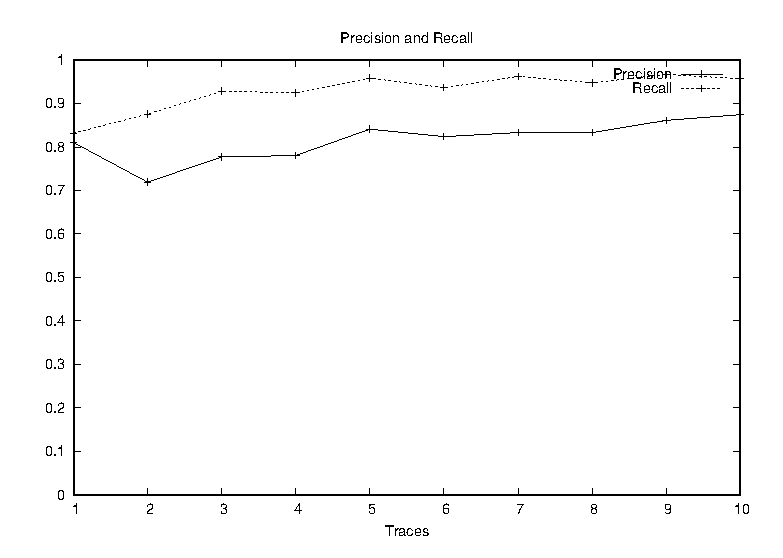
\includegraphics[width=0.65\linewidth]{figures/input_size_100_10_precision.eps}
	\caption{Precision and Recall when learning from [1-10] plan traces with \FO action sequences and \PO state trajectories with 10\% observability.}
	\label{fig:np_quality}
\end{figure}

\begin{figure}[hbt!]
	\centering
	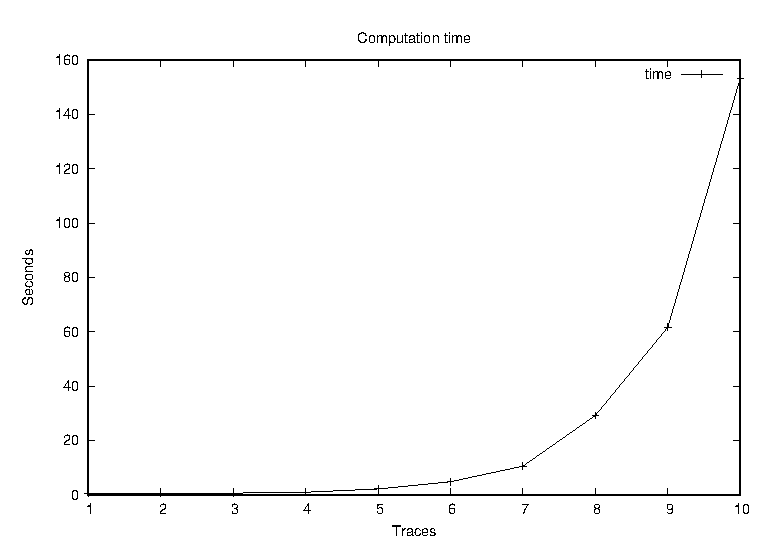
\includegraphics[width=0.65\linewidth]{figures/input_size_100_10_time.eps}
	\caption{Computation time when learning from [1-10] plan traces with \FO action sequences and \PO state trajectories with 10\% observability.}
	\label{fig:np_time}
\end{figure}

Figure~\ref{fig:pspace_quality} displays the quality of the learned models in the PSPACE-complete scenario. As expectedly, the values of Precision and Recall are lower than in the NP-complete case. We can also observe in Figure~\ref{fig:pspace_quality} the opposite behaviour to Figure~\ref{fig:np_quality}; that is, we find a drop of the quality as the input knowledge increases. The drop in the score is caused by an increasing number of timeouts, meaning that no solution is found in many tasks within the given time-bound, and consequently a value of $0$ for Precision and Recall is assigned to these experiments. Figure \ref{fig:pspace_time}, on the other hand, reflects that the computation time of the PSPACE-complete scenario is also higher than the NP-complete scenario, which is again explained by the large number of timeouts.


The conclusions we draw from these experiments is that learning with few input samples yield action models that are fairly sound and almost totally complete in the NP-complete scenario and less accurate in the PSPACE-complete scenarios. In the latter, while being timeouts the main cause of the drop in the score, we must point out that pure syntax-based metrics are not adequate to evaluate such under-constrained tasks since the phenomenon of \emph{reformulation} occurs and this largely impacts the results. We will provide experimental evidence of this in section \ref{minimal}.


%For the PSPACE-complete scenario, {\em precision} and {\em recall} scores have to be taken with a grain of salt because {\bf pure syntax-based metrics are not informative when reformulations appear} (we provide experimental evidence of this in Section \ref{minimal}).



\begin{figure}[hbt!]
	\centering
	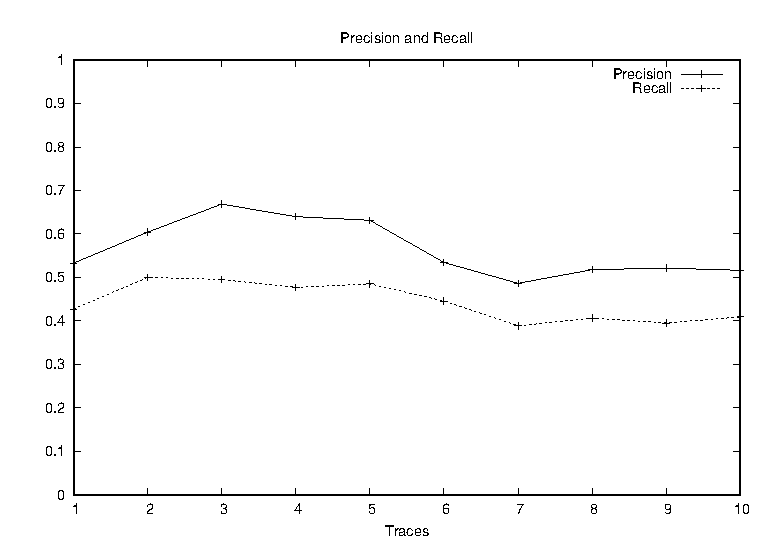
\includegraphics[width=0.65\linewidth]{figures/input_size_0_0_precision.eps}
	\caption{Precision and Recall when learning from [1-10] plan traces with \NO action sequences and \NO state trajectories.}
	\label{fig:pspace_quality}
\end{figure}
\begin{figure}[hbt!]
	\centering
	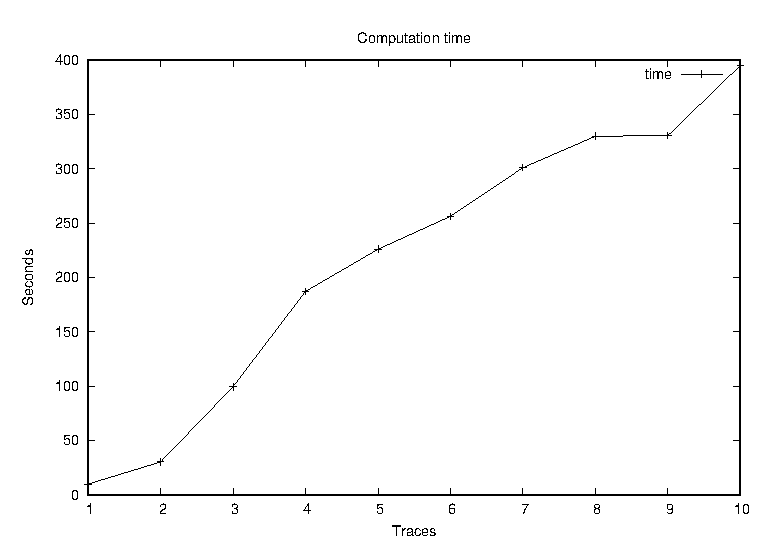
\includegraphics[width=0.65\linewidth]{figures/input_size_0_0_time.eps}
	\caption{Computation time when learning from [1-10] plan traces with \NO action sequences and \NO state trajectories.}
	\label{fig:pspace_time}
\end{figure}

%The conclusion we can draw is that learning from few input samples is both our strong point and our limitation. Results on the NP-complete scenario show that the learned models are considerably sound and complete (to put these results into a richer perspective we will also compare ourselves with another approach in the following section). The PSPACE-complete scenario, on the other hand, shows that the learned models have less quality. Nevertheless, we argue that syntax-based metrics are not appropriate for the PSPACE-complete scenario due to the vast amount of reformulations that can appear in such under-constrained learning task and we will show proof of this in section \ref{minimal}.


\subsection{Comparison with \ARMS}

In this section we analyze the performance of \FAMA compared to \ARMS, one of the most well-known approaches to learning planning models. \ARMS, as well as most of the existing current learning systems, works under the assumption of plan traces with \FO action sequences and \NO state trajectories and therefore is not able to handle the PSPACE-complete scenario. We will thereby restrict the experimentation to the cases manageable by \ARMS.

In this experiment, we defined a \emph{degree of observability} $\sigma$ for the state trajectory, ranging from 0\% to 100\%, that measures the probability of observing a literal, and evaluated both \FAMA and \ARMS for increasing values of $\sigma$ using five traces as input knowledge. When $\sigma = 0$ we have a \NO state trajectory, when $\sigma=100$ we have a \FO state trajectory and all cases in-between correspond to the \PO scenario.

Figures \ref{fig:comparison_precision} and \ref{fig:comparison_recall} compare \FAMA and \ARMS in terms of Precision and Recall. The horizontal axes represent the degree of observability and vertical axes show the average Precision (Figure \ref{fig:comparison_precision}) and Recall (Figure \ref{fig:comparison_recall}) computed over the 14 tested domains. Remarkably, \FAMA dominates in terms of Precision in all cases except for the \FO state trajectories. Particularly, the models learned by \FAMA are between 15\% to 24\% more precise than those learned by \ARMS. A similar trend is observed for Recall (Figure \ref{fig:comparison_recall}), where the difference is even larger, meaning that our learned models are more complete.

The results highlight that \FAMA outperforms \ARMS when very few plan traces are available. This by no means is conclusive that \FAMA is overall better in NP-complete scenarios but only that is able to learn better with very limited input knowledge (actually, Figure~\ref{fig:np_time} reflects the exponential behaviour of \FAMA with more than five traces).



\begin{figure}[hbt!]
	\centering
	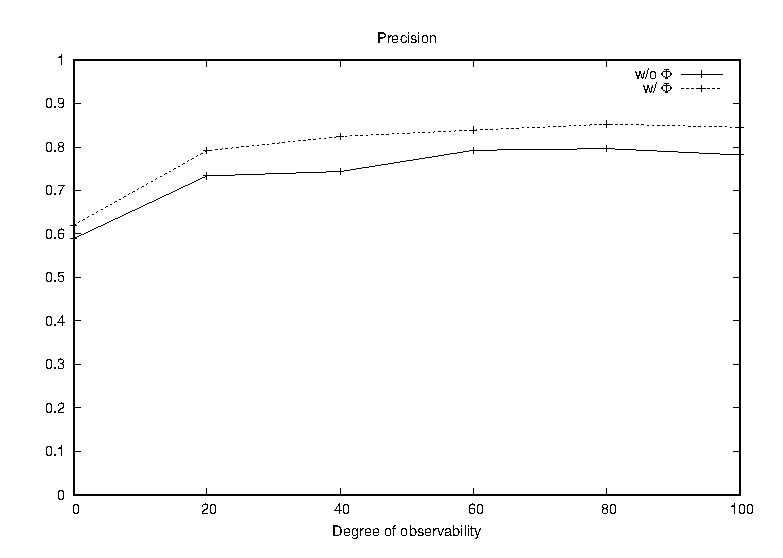
\includegraphics[width=.65\linewidth]{figures/comparison_precision.eps}
	\caption{Precision comparison between \FAMA and \ARMS for different \emph{degrees of observability}.}
	\label{fig:comparison_precision}
\end{figure}

\begin{figure}[hbt!]
	\centering
	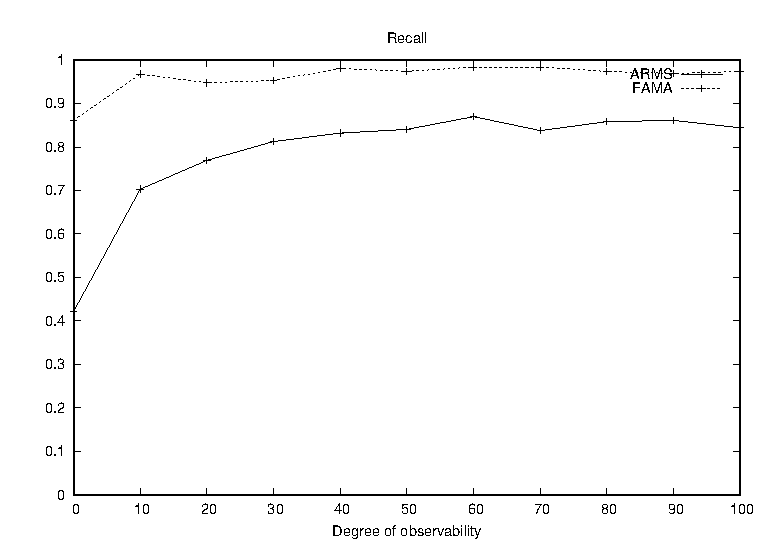
\includegraphics[width=.65\linewidth]{figures/comparison_recall.eps}
	\caption{Recall comparison between \FAMA and \ARMS for different \emph{degrees of observability}.}
	\label{fig:comparison_recall}
\end{figure}



%Remarkably, the overall \emph{precision} is now $0.98$, which means that the contents of the learned models is highly reliable. The value of \emph{recall}, 0.87, is an indication that the learned models still miss some information (preconditions are again the component more difficult to be fully learned). Overall, the results confirm the previous trend: the more input knowledge of the task, the better the models and the less planning time. Additionally, the solution plans required for this task are smaller because it is only necessary to program half of the actions (the other half are included in the input knowledge $\mathcal{M}$). {\em Visitall} and {\em Hanoi} are excluded from this evaluation because they only contain one action schema.


\subsection{Learning with minimal input knowledge}
\label{minimal}

%In the previous experiments we have given a general view of the performance of \FAMA under different conditions. So far, experiments have shown that \FAMA is able to learn with very small amounts of input knowledge, be it due to low observability or few training samples.

In this section, we will take a closer look at the action models learned from minimal input knowledge. To that end, we will limit the input to only two plan traces and analyze the results under different degrees of observability. We evaluate three case studies, the first one is an NP-complete scenario and the other two are PSPACE-complete:

\begin{itemize}
	\item \textbf{\FO action sequence and \PO state trajectory}: We are, once again, assuming a degree of observability of 10\% for the state trajectory. Results of this case study are detailed in Table \ref{tab:results_minimum_100_10}.
	\item  \textbf{\PO action sequence and \PO state trajectory}: In this case study we are assuming a degree of observability of 30\% for both the action sequence and state trajectory. Results are shown in Table \ref{tab:results_minimum_30_30}.
	\item  \textbf{\NO action sequence and \NO state trajectory}: Both the action sequence and state trajectory are completely empty so only the initial and final states are observed; i.e., $\tau = \tup{s_0, s_m}, \forall \tau \in \mathcal{T}$. Results of this case study are reported in Table \ref{tab:results_minimum_0_0}.
\end{itemize}

All tables in this section (Tables \ref{tab:results_minimum_100_10}, \ref{tab:results_minimum_30_30} and \ref{tab:results_minimum_0_0}) follow the same structure. Precision ({\bf P}) and Recall ({\bf R}) scores are computed separately for the preconditions ({\bf Pre}), positive effects ({\bf Add}) and negative Effects ({\bf Del}), and also globally ({\bf Global}). The last column reports the computation time (in seconds) needed to obtain the learned models. Missing values in the tables (reported as -) correspond to domains where no solution was found within a 1800s timeout.

Table \ref{tab:results_minimum_100_10} shows the results of the first case study. Recall scores are generally higher than the precision ones, and, in fact, the models learned for six out of the 14 domains were perfectly complete. Although precision is overall lower, it is interesting to notice that the learned sets of negative effects are mostly flawless. With regards to the computation time, we can observe times are below one second in all cases except for the {\em floor-tile} domain.

\begin{table}[hbt!]
		\begin{center}
                  \begin{footnotesize}			
			\begin{tabular}{l|l|l|l|l|l|l||l|l||l|}
				& \multicolumn{2}{|c|}{\bf Pre} & \multicolumn{2}{|c|}{\bf Add} & \multicolumn{2}{|c||}{\bf Del} & \multicolumn{2}{|c|}{\bf Global} & \\ \cline{2-9}			
				& \multicolumn{1}{|c|}{\bf P} & \multicolumn{1}{|c|}{\bf R} & \multicolumn{1}{|c|}{\bf P} & \multicolumn{1}{|c|}{\bf R} & \multicolumn{1}{|c|}{\bf P} & \multicolumn{1}{|c||}{\bf R} &  \multicolumn{1}{|c|}{\bf P} & \multicolumn{1}{|c|}{\bf R} & {\bf Time} \\
				\hline
				blocks & 0.86 & 0.67 & 0.86 & 0.67 & 0.8 & 0.44 & 0.84 & 0.59& 0.21 \\ % [(u'pick-up', u'pick-up', 1), (u'put-down', u'put-down', 1), (u'stack', u'stack', 1, 2), (u'unstack', u'unstack', 1, 2)]
				driverlog & 0.68 & 0.93 & 0.5 & 0.57 & 0.83 & 0.71 & 0.67 & 0.79& 0.27 \\ % [(u'load-truck', u'load-truck', 1, 2, 3), (u'unload-truck', u'unload-truck', 1, 2, 3), (u'board-truck', u'board-truck', 1, 2, 3), (u'disembark-truck', u'disembark-truck', 1, 2, 3), (u'walk', u'walk', 1, 2, 3), (u'drive-truck', u'drive-truck', 1, 2, 3, 4)]
				ferry & 0.78 & 1.0 & 0.5 & 1.0 & 1.0 & 1.0 & 0.71 & 1.0& 0.4 \\ % [(u'sail', u'sail', 1, 2), (u'board', u'board', 1, 2), (u'debark', u'debark', 1, 2)]
				floor-tile & 0.69 & 1.0 & 0.45 & 0.91 & 1.0 & 0.82 & 0.65 & 0.93& 1.42 \\ % [(u'change-color', u'change-color', 1, 2, 3), (u'up', u'up', 1, 2, 3), (u'down', u'down', 1, 2, 3), (u'right', u'right', 1, 2, 3), (u'left', u'left', 1, 2, 3), (u'paint-up', u'paint-up', 1, 2, 3, 4), (u'paint-down', u'paint-down', 1, 2, 3, 4)]
				grid & 0.76 & 0.94 & 0.55 & 0.86 & 1.0 & 1.0 & 0.74 & 0.94& 0.7 \\ % [(u'move', u'move', 1, 2), (u'pickup', u'pickup', 1, 2), (u'putdown', u'putdown', 1, 2), (u'pickup-and-loose', u'pickup-and-loose', 1, 2, 3), (u'unlock', u'unlock', 1, 2, 3, 4)]
				gripper-strips & 1.0 & 1.0 & 1.0 & 1.0 & 1.0 & 1.0 & 1.0 & 1.0& 0.16 \\ % [(u'move', u'move', 1, 2), (u'pick', u'pick', 1, 2, 3), (u'drop', u'drop', 1, 2, 3)]
				hanoi & 0.67 & 1.0 & 0.67 & 1.0 & 1.0 & 1.0 & 0.73 & 1.0& 0.31 \\ % [(u'move', u'move', 1, 2, 3)]
				miconic & 1.0 & 1.0 & 0.5 & 1.0 & 1.0 & 1.0 & 0.8 & 1.0& 0.29 \\ % [(u'board', u'board', 1, 2), (u'depart', u'depart', 1, 2), (u'up', u'up', 1, 2), (u'down', u'down', 1, 2)]
				n-puzzle & 0.75 & 1.0 & 1.0 & 1.0 & 1.0 & 1.0 & 0.88 & 1.0& 0.28 \\ % [(u'move', u'move', 1, 2, 3)]
				parking & 0.73 & 0.79 & 0.7 & 0.78 & 1.0 & 0.78 & 0.78 & 0.78& 0.65 \\ % [(u'move-curb-to-curb', u'move-curb-to-curb', 1, 2, 3), (u'move-curb-to-car', u'move-curb-to-car', 1, 2, 3), (u'move-car-to-curb', u'move-car-to-curb', 1, 2, 3), (u'move-car-to-car', u'move-car-to-car', 1, 2, 3)]
				satellite & 0.93 & 1.0 & 0.63 & 1.0 & 1.0 & 0.75 & 0.85 & 0.96& 0.36 \\ % [(u'switch-on', u'switch-on', 1, 2), (u'switch-off', u'switch-off', 1, 2), (u'turn-to', u'turn-to', 1, 2, 3), (u'calibrate', u'calibrate', 1, 2, 3), (u'take-image', u'take-image', 1, 2, 3, 4)]
				transport & 1.0 & 1.0 & 0.71 & 1.0 & 1.0 & 0.6 & 0.9 & 0.9& 0.22 \\ % [(u'drive', u'drive', 1, 2, 3), (u'pick-up', u'pick-up', 1, 2, 3, 4, 5), (u'drop', u'drop', 1, 2, 3, 4, 5)]
				grid-visit-all & 0.67 & 1.0 & 0.5 & 1.0 & 1.0 & 1.0 & 0.63 & 1.0& 0.87 \\ % [(u'move', u'move', 1, 2)]
				zeno-travel & 0.92 & 0.79 & 0.6 & 0.86 & 0.8 & 0.57 & 0.78 & 0.75& 0.26 \\ % [(u'board', u'board', 1, 2, 3), (u'debark', u'debark', 1, 2, 3), (u'refuel', u'refuel', 1, 2, 3, 4), (u'fly', u'fly', 1, 2, 3, 4, 5), (u'zoom', u'zoom', 1, 2, 3, 4, 5, 6)]
				\hline
				\bf & 0.82 & 0.94 & 0.66 & 0.90 & 0.96 & 0.83 & 0.78 & 0.90 & 0.46 \\
			\end{tabular}
                  \end{footnotesize}			
		\end{center}
	\caption{\small {\em Precision} and {\em recall} scores for learning tasks with \FO action sequences and \PO state trajectories with 10\% observability.}
	\label{tab:results_minimum_100_10}
\end{table}


Table \ref{tab:results_minimum_30_30} gathers the results of the PSPACE-complete case study with 30\% observability.  We can see in the table that the scores of some domains are missing. This is the case of {\em floor-tile} and {\em parking}, which not only are fairly complex domains, but also categorized as \emph{puzzle-like} domains, a feature that is known for putting a strain in the planners. Interestingly enough, we note the huge computation time of {\em hanoi}, which also qualifies as a \emph{puzzle-like} domain. Regarding quality, we find that the learned models retain a level of soundness similar to Table~\ref{tab:results_minimum_100_10} but the completeness is lower than in the previous case study. This is specially noticeable in the preconditions, where recall values drop from from 0.94 to 0.54. This is because the input actions act as strong constraints playing a key role on the closeness of the learned model to the GTM. The more actions are missing in the input knowledge, the more likely the occurrence of reformulations.

\begin{table}[hbt!]
	\begin{center}
		\begin{footnotesize}
		\begin{tabular}{l|l|l|l|l|l|l||l|l||l|}
			& \multicolumn{2}{|c|}{\bf Pre} & \multicolumn{2}{|c|}{\bf Add} & \multicolumn{2}{|c||}{\bf Del} & \multicolumn{2}{|c|}{\bf Global} & \\ \cline{2-9}			
			& \multicolumn{1}{|c|}{\bf P} & \multicolumn{1}{|c|}{\bf R} & \multicolumn{1}{|c|}{\bf P} & \multicolumn{1}{|c|}{\bf R} & \multicolumn{1}{|c|}{\bf P} & \multicolumn{1}{|c||}{\bf R} &  \multicolumn{1}{|c|}{\bf P} & \multicolumn{1}{|c|}{\bf R} & {\bf Time} \\
			\hline
			blocks & 1.0 & 0.89 & 0.9 & 1.0 & 1.0 & 0.89 & 0.96 & 0.93& 3.51 \\ % [(u'pick-up', u'put-down', 1), (u'put-down', u'pick-up', 1), (u'stack', u'stack', 1, 2), (u'unstack', u'unstack', 1, 2)]
			driverlog & 0.3 & 0.21 & 0.31 & 0.57 & 0.29 & 0.29 & 0.3 & 0.32& 24.41 \\ % [(u'load-truck', u'unload-truck', 1, 2, 3), (u'unload-truck', u'load-truck', 1, 2, 3), (u'board-truck', u'board-truck', 1, 2, 3), (u'disembark-truck', u'disembark-truck', 1, 2, 3), (u'walk', u'walk', 2, 1, 3), (u'drive-truck', u'drive-truck', 1, 2, 3, 4)]
			ferry & 0.83 & 0.71 & 0.8 & 1.0 & 1.0 & 1.0 & 0.87 & 0.87& 4.39 \\ % [(u'sail', u'sail', 1, 2), (u'board', u'board', 1, 2), (u'debark', u'debark', 1, 2)]
			floor-tile & - & - & - & - & - & - & - & - & - \\ % [(u'change-color', u'change-color', 1, 2, 3), (u'up', u'change-color', 1, 3, 2), (u'down', u'up', 1, 2, 3), (u'right', u'up', 1, 3, 2), (u'left', u'down', 1, 3, 2), (u'paint-up', u'paint-up', 1, 2, 3, 4), (u'paint-down', u'paint-down', 1, 2, 3, 4)]
			grid & - & - & - & - & - & - & - & - & - \\ % [(u'move', u'move', 1, 2), (u'pickup', u'move', 2, 1), (u'putdown', u'putdown', 1, 2), (u'pickup-and-loose', u'pickup-and-loose', 1, 2, 3), (u'unlock', u'unlock', 1, 2, 3, 4)]
			gripper-strips & 1.0 & 0.67 & 0.8 & 1.0 & 1.0 & 1.0 & 0.92 & 0.86& 1.31 \\ % [(u'move', u'move', 1, 2), (u'pick', u'pick', 1, 2, 3), (u'drop', u'drop', 1, 2, 3)]
			hanoi & 1.0 & 0.5 & 1.0 & 1.0 & 1.0 & 1.0 & 1.0 & 0.75& 1566.44 \\ % [(u'move', u'move', 1, 2, 3)]
			miconic & 0.75 & 0.33 & 0.5 & 0.75 & 0.5 & 0.67 & 0.57 & 0.5& 0.86 \\ % [(u'board', u'board', 1, 2), (u'depart', u'depart', 1, 2), (u'up', u'up', 2, 1), (u'down', u'down', 1, 2)]
			n-puzzle & 1.0 & 1.0 & 1.0 & 1.0 & 1.0 & 1.0 & 1.0 & 1.0& 62.82 \\ % [(u'move', u'move', 1, 2, 3)]
			parking & - & - & - & - & - & - & - & - & - \\ % [(u'move-curb-to-curb', u'move-curb-to-curb', 1, 2, 3), (u'move-curb-to-car', u'move-curb-to-curb', 1, 3, 2), (u'move-car-to-curb', u'move-curb-to-car', 1, 2, 3), (u'move-car-to-car', u'move-car-to-curb', 1, 2, 3)]
			satellite & 0.78 & 0.5 & 0.57 & 0.8 & 0.33 & 0.25 & 0.63 & 0.52& 22.76 \\ % [(u'switch-on', u'switch-on', 1, 2), (u'switch-off', u'switch-off', 1, 2), (u'turn-to', u'turn-to', 1, 2, 3), (u'calibrate', u'calibrate', 1, 2, 3), (u'take-image', u'take-image', 1, 2, 3, 4)]
			transport & 0.5 & 0.3 & 0.43 & 0.6 & 0.5 & 0.4 & 0.47 & 0.4& 31.07 \\ % [(u'drive', u'drive', 1, 2, 3), (u'pick-up', u'pick-up', 1, 2, 3, 5, 4), (u'drop', u'drop', 1, 2, 3, 5, 4)]
			grid-visit-all & 1.0 & 0.5 & 0.5 & 0.5 & 1.0 & 1.0 & 0.75 & 0.6& 3.11 \\ % [(u'move', u'move', 1, 2)]
			zeno-travel & 0.67 & 0.29 & 0.75 & 0.43 & 0.75 & 0.43 & 0.71 & 0.36& 494.2 \\ % [(u'board', u'board', 1, 2, 3), (u'debark', u'debark', 1, 2, 3), (u'refuel', u'refuel', 1, 2, 3, 4), (u'fly', u'fly', 1, 3, 2, 5, 4), (u'zoom', u'zoom', 1, 2, 3, 4, 5, 6)]
			\hline
			\bf & 0.80 & 0.54 & 0.69 & 0.79 & 0.76 & 0.72 & 0.74 & 0.65 & 201.35
			
		\end{tabular}
		\end{footnotesize}
	\end{center}
	\caption{\small {\em Precision} and {\em recall} when learning with \PO action sequences and \PO state trajectories, 30\% observability in both cases.}
	\label{tab:results_minimum_30_30}
\end{table}


We now analyze the PSPACE case study with \NO action sequences and \NO state trajectories (Table~\ref{tab:results_minimum_0_0}). A first outstanding observation is that, contrary to what might be expected by looking at the previous table, we are able in this case to find solutions for all the domains. This happens because the search is less constrained and consequently there are far more possible solutions for this learning task. This broader space of solutions is also stressed in a diminished quality of the learned models. Thus, despite the learned models are compliant with the input data, they are further from the original GTM. In Table~\ref{tab:results_minimum_0_0} we can observe the global values of Precision and Recall drop to 0.6 and 0.5, respectively.

We argue, however, that syntax-based metrics are not appropriate for scenarios with minimal observability as they cannot cope with the reformulations that frequently occur in these circumstances. To illustrate this, Figure \ref{fig:macroaction} shows the PDDL encoding of the action model of the {\tt\small stack} operator learned from plan traces with \NO action sequences and \NO state trajectories. This learned action model removes a block from on top of another block and puts it down on the table in a single step. There are two main differences with respect to the model of the {\tt\small stack} operator of the GTM: (1) the learned action is actually \emph{unstacking} a block instead of stacking it and (2) the block on the top ends on the table, not held by the robot arm. We refer to the first difference as \emph{role swapping} and it happens when there are missing actions in the input plan trace. If no actions are present in the input traces, the names of actions become meaningless, in which case the effectively anonymous actions can interchange their behaviour with any other comparable action model. The second difference indeed reveals that the learned action model is working as an {\tt\small unstack+put-down} \emph{macro-action}. This happens when there are missing states in the input traces since a \emph{macro-action} can be seen as the application of more than one action in a single step, thus skipping some intermediate states.

Reformulated action models, like the one in Figure \ref{fig:macroaction}, are indeed sound models that can be used to solve planning tasks. For instance, any \emph{blocks-world} problem can be solved unstacking all the blocks to the table ({\tt\small unstack+put-down}) and then stacking them to meet the goal conditions ({\tt\small pick-up+stack}). Hence, the \NO/\NO case study features all the conditions for reformulation to happen, and this is the reason why scenarios such as this one are better evaluated using {\em semantic-based metrics}.


\begin{table}[hbt!]
  \begin{center}
    \begin{footnotesize}
		\begin{tabular}{l|l|l|l|l|l|l||l|l||l|}
			& \multicolumn{2}{|c|}{\bf Pre} & \multicolumn{2}{|c|}{\bf Add} & \multicolumn{2}{|c||}{\bf Del} & \multicolumn{2}{|c|}{\bf Global} & \\ \cline{2-9}			
			& \multicolumn{1}{|c|}{\bf P} & \multicolumn{1}{|c|}{\bf R} & \multicolumn{1}{|c|}{\bf P} & \multicolumn{1}{|c|}{\bf R} & \multicolumn{1}{|c|}{\bf P} & \multicolumn{1}{|c||}{\bf R} &  \multicolumn{1}{|c|}{\bf P} & \multicolumn{1}{|c|}{\bf R} & {\bf Time} \\
			\hline
			blocks & 0.5 & 0.56 & 0.5 & 0.33 & 0.75 & 0.33 & 0.55 & 0.41& 0.27 \\ % [(u'pick-up', u'put-down', 1), (u'put-down', u'pick-up', 1), (u'stack', u'stack', 1, 2), (u'unstack', u'unstack', 1, 2)]
			driverlog & 0.13 & 0.07 & 0.38 & 0.71 & 0.0 & 0.0 & 0.25 & 0.21& 0.98 \\ % [(u'load-truck', u'load-truck', 1, 2, 3), (u'unload-truck', u'unload-truck', 1, 2, 3), (u'board-truck', u'disembark-truck', 1, 2, 3), (u'disembark-truck', u'board-truck', 1, 2, 3), (u'walk', u'walk', 1, 2, 3), (u'drive-truck', u'drive-truck', 1, 2, 3, 4)]
			ferry & 0.5 & 0.29 & 0.5 & 0.5 & 0.67 & 0.5 & 0.55 & 0.4& 0.47 \\ % [(u'sail', u'sail', 1, 2), (u'board', u'board', 1, 2), (u'debark', u'debark', 1, 2)]
			floor-tile & 0.34 & 0.64 & 0.5 & 0.36 & 0.44 & 0.73 & 0.39 & 0.59& 165.92 \\ % [(u'change-color', u'change-color', 1, 2, 3), (u'up', u'up', 1, 3, 2), (u'down', u'left', 1, 2, 3), (u'right', u'right', 1, 3, 2), (u'left', u'left', 1, 3, 2), (u'paint-up', u'paint-up', 1, 3, 2, 4), (u'paint-down', u'paint-down', 1, 3, 2, 4)]
			grid & 0.47 & 0.41 & 0.38 & 0.43 & 0.25 & 0.29 & 0.39 & 0.39& 214.87 \\ % [(u'move', u'move', 1, 2), (u'pickup', u'pickup', 1, 2), (u'putdown', u'putdown', 1, 2), (u'pickup-and-loose', u'pickup-and-loose', 1, 3, 2), (u'unlock', u'unlock', 2, 1, 3, 4)]
			gripper-strips & 1.0 & 0.83 & 1.0 & 1.0 & 1.0 & 1.0 & 1.0 & 0.93& 0.2 \\ % [(u'move', u'move', 1, 2), (u'pick', u'pick', 1, 2, 3), (u'drop', u'drop', 1, 2, 3)]
			hanoi & 0.6 & 0.75 & 1.0 & 1.0 & 1.0 & 1.0 & 0.78 & 0.88& 3.23 \\ % [(u'move', u'move', 1, 3, 2)]
			miconic & 0.4 & 0.44 & 0.6 & 0.75 & 0.25 & 0.33 & 0.42 & 0.5& 0.25 \\ % [(u'board', u'board', 1, 2), (u'depart', u'depart', 1, 2), (u'up', u'up', 2, 1), (u'down', u'down', 2, 1)]
			n-puzzle & 1.0 & 1.0 & 1.0 & 1.0 & 1.0 & 1.0 & 1.0 & 1.0& 4.15 \\ % [(u'move', u'move', 1, 2, 3)]
			parking & 0.67 & 0.57 & 0.43 & 0.33 & 0.5 & 0.44 & 0.56 & 0.47& 7.61 \\ % [(u'move-curb-to-curb', u'move-curb-to-curb', 1, 3, 2), (u'move-curb-to-car', u'move-curb-to-car', 1, 2, 3), (u'move-car-to-curb', u'move-car-to-curb', 1, 2, 3), (u'move-car-to-car', u'move-car-to-car', 2, 1, 3)]
			satellite & 0.5 & 0.14 & 0.5 & 0.6 & 0.75 & 0.75 & 0.57 & 0.35& 2.06 \\ % [(u'switch-on', u'switch-on', 1, 2), (u'switch-off', u'switch-off', 1, 2), (u'turn-to', u'turn-to', 1, 3, 2), (u'calibrate', u'calibrate', 1, 2, 3), (u'take-image', u'take-image', 1, 2, 3, 4)]
			transport & 0.6 & 0.3 & 0.38 & 0.6 & 0.5 & 0.2 & 0.47 & 0.35& 0.83 \\ % [(u'drive', u'drive', 1, 3, 2), (u'pick-up', u'drop', 1, 2, 3, 4, 5), (u'drop', u'pick-up', 1, 2, 3, 4, 5)]
			grid-visit-all & 0.0 & 0.0 & 1.0 & 0.5 & 0.0 & 0.0 & 1.0 & 0.2& 1.24 \\ % [(u'move', u'move', 2, 1)]
			zeno-travel & 0.86 & 0.43 & 0.29 & 0.29 & 0.33 & 0.14 & 0.53 & 0.32& 28.4 \\ % [(u'board', u'debark', 1, 2, 3), (u'debark', u'board', 1, 2, 3), (u'refuel', u'refuel', 1, 2, 3, 4), (u'fly', u'fly', 1, 2, 3, 4, 5), (u'zoom', u'zoom', 1, 2, 3, 5, 6, 4)]
			\hline
			\bf & 0.54 & 0.46 & 0.60 & 0.60 & 0.53 & 0.48 & 0.60 & 0.50 & 30.75
		\end{tabular}
            \end{footnotesize}
	\end{center}
	\caption{\small {\em Precision} and {\em recall} scores for learning tasks with \NO action sequences and \NO state trajectories.}
	\label{tab:results_minimum_0_0}
\end{table}


\begin{figure}[hbt!]
	\begin{footnotesize}
		\begin{verbatim}
(:action stack
 :parameters (?o1 - object ?o2 - object)
 :precondition (and (on ?o1 ?o2)(handempty ))
 :effect (and (not (on ?o1 ?o2))(clear ?o1)(clear ?o2)(ontable ?o1)))
		\end{verbatim}
	\end{footnotesize}
	\caption{PDDL encoding of the learned action model of the {\em stack} operator from the four-operator {\em blocksworld} domain.}
	\label{fig:macroaction}
\end{figure}



\subsection{Syntactic versus semantic evaluation}

Our last experiment is devoted to compare the scores provided by the syntactic and semantic versions of Precision and Recall. For that purpose, we will evaluate the models learned in Section \ref{minimal} both syntactically, using the GTM, and semantically, computing the set of action models closest to the learned models that is compliant with a testing set of five traces (see Definition \ref{compliant}). We must note that since we are using {\sc Madagascar}, a satisficing planner, the solution to the model evaluation may not be the closest compliant model, reason why the scores of sem-Precision and sem-Recall are approximate values. Our goal with this experiment is to gauge the suitability of the semantic metrics proposed in section \ref{sec:evaluation} with respect to their well-known counterparts. With that in mind, we define two case studies:

\begin{itemize}
	\item \textbf{\FO action sequence and \PO state trajectory}: In this case study the full sequence of actions is known and no states are missing, which makes it practically impossible for reformulated models to appear. In fact, in all our experimentation with \FAMA and other approaches we never observed reformulations when the full sequence of actions is known.
	\item  \textbf{\NO action sequence and \NO state trajectory}: This is a case study that favors reformulations in the learned models, as previously discussed.
\end{itemize}

\begin{table}[hbt!]
     \begin{footnotesize}
	\begin{center}		
		\begin{tabular}{l|c|c|c|c|}		
			& {\bf Precision} & {\bf Recall} & {\bf sem-Precision} & {\bf sem-Recall} \\
			\hline
			blocks & 0.84 & 0.59 & 0.84 & 0.64 \\
			driverlog & 0.67 & 0.79 & 0.70 & 0.92 \\
			ferry & 0.71 & 1.0 & 1.0 & 1.0 \\
			floor-tile & 0.65 & 0.93 & 0.95 & 0.95 \\
			grid & 0.74 & 0.94 & 1.0 & 0.98 \\
			gripper-strips & 1.0 & 1.0 & 1.0 & 1.0 \\
			hanoi & 0.73 & 1.0 & 0.91 & 1.0 \\
			miconic & 0.8 & 1.0	& 1.0 & 1.0 \\
			n-puzzle & 0.88 & 1.0 & 1.0 & 1.0 \\
			parking & 0.78 & 0.78 & 0.97 & 0.84 \\
			satellite & 0.85 & 0.96 & 0.96 & 1.0 \\
			transport & 0.9 & 0.9 & 1.0 & 1.0 \\
			grid-visit-all & 0.63 & 1 & 1.0 & 1.0 \\
			zeno-travel & 0.78 & 0.75 & 0.85 & 0.96 \\
			\hline
			& 0.78 & 0.9 & 0.94 & 0.95
		\end{tabular}
	\end{center}
     \end{footnotesize}
     \caption{\small Syntactic and semantic scores when learning with \FO action sequences and \PO state trajectories with 10\% observability.}
     \label{tab:metric_comparison_100_10}
\end{table}


Table \ref{tab:metric_comparison_100_10} shows the results of the first case study. Looking at the high scores of the syntactic metrics, specially the value of Recall, we can conclude that the learned models are, in fact, fairly similar to the GTM. This supports our conclusion that no reformulation occurs in this case study, which also means that the space of possible solutions is restricted to models close to the GTM. The values of sem-Precision and sem-Recall are also very high across the table, which is exactly the desired behavior for these metrics given that solutions are very close to the GTM. In comparison, Recall and sem-Recall show similar scores, while sem-Precision is significantly higher than Precision, thus showing that the sem-Precision is more lenient towards extra preconditions or effects. This is in line with the results of the previous experiments, where the common appearance of redundant or implicit preconditions in the learned models is penalized by the Precision metric. We can interpret this phenomenon as a manifestation of the qualification problem~\cite{GinsbergS88}. For instance, the model learned for the {\tt\small move} action of the {\em hanoi} domain specifies that both the origin and destination disks must be bigger than the one moving, but the GTM contains only one of these preconditions. This learned model is semantically correct but syntactically different from the GTM and hence penalized by the Precision metric.

Table~\ref{tab:metric_comparison_0_0} details the results of the \NO/\NO case study. One first observation is the impossibility of applying a semantic evaluation in some of the most complex domains with five traces. Contrary to the previous case study, the difference between the syntactic and semantic metrics is larger in this PSPACE-complete scenario. Comparing the scores of both versions, we find that learned models that achieved mediocre scores when using the GTM as reference (syntactic metrics), are in fact reasonably sound and complete, reaching an overall score of 0.91 in both sem-Precision and sem-Recall. This is an indication that the models learned by our approach, despite syntactically different from the GTM, require very few editions to explain the testing set of traces.

\begin{table}[hbt!]
     \begin{footnotesize}
	\begin{center}		
		\begin{tabular}{l|c|c|c|c|}		
			& {\bf Precision} & {\bf Recall} & {\bf sem-Precision} & {\bf sem-Recall} \\
			\hline
			blocks & 0.55 & 0.41 & 0.9 & 0.86 \\
			driverlog & 0.25 & 0.21 & 0.54 & 0.72 \\
			ferry & 0.55 & 0.4 & 1.0 & 0.79 \\
			floor-tile & 0.39 & 0.59 & - & - \\
			grid & 0.39 & 0.39 & - & - \\
			gripper-strips & 1.0 & 0.93 & 1.0 & 1.0 \\
			hanoi & 0.78 & 0.88 & 0.89 & 1.0 \\
			miconic & 0.42 & 0.5 & 0.89 & 0.85 \\
			n-puzzle & 1.0 & 1.0 & 1.0 & 1.0 \\
			parking & 0.56 & 0.47 & - & - \\
			satellite & 0.57 & 0.35 & - & - \\
			transport & 0.47 & 0.35 & 0.93 & 0.93 \\
			grid-visit-all & 1.0 & 0.2 & 1.0 & 1.0 \\
			zeno-travel & 0.53 & 0.32 & - & - \\
			\hline
			& 0.6 & 0.5 & 0.91 & 0.91
		\end{tabular}
	\end{center}
        \end{footnotesize}
	\caption{\small Syntactic and semantic metric scores for learning tasks with \NO action sequences and \NO state trajectories.}
	\label{tab:metric_comparison_0_0}
\end{table}

Looking at the results of both case studies we can draw two conclusions with regards to the semantic metrics proposed in this paper. The first one is that, when no reformulation occurs, these metrics behave similarly to their syntactic counterparts, which means they are a good substitute when the GTM is not available. The second conclusion is that sem-Precision and sem-Recall are better suited to evaluate reformulated models than the original syntactic metrics since they contemplate valid solutions outside the GTM that successfully explain the given input data.



\section{Conclusions}
\label{sec:Section9}
We presented a novel approach for learning \strips\ action models from examples using classical planning. The approach is flexible to various amount and kind of input knowledge and accepts partially specified action models. Unlike extensive-data ML approaches, our work explores an alternative research direction to learn sound models from very small data sets. The action models of the {\em blocksworld} or {\em gripper} domains were perfectly learned from only 25 state observations. Moreover, in 12 out of the 15 domains, the learned models yield {\em Precision} values over $0.75$.

To the best of our knowledge, this is the first work on learning \strips\ action models from state observations, using exclusively an {\em off-the-shelf} classical planner, and evaluated over a wide range of different domains. Recently, the work in~\cite{SternJ17} proposes a planning compilation for learning action models from plan traces following the {\em finite domain} representation for the state variables. This is a theoretical study on the boundaries of the learned models and no experimental results are reported.

We also introduced the {\em precision} and {\em recall} metrics, widely used in ML, for evaluating the learned action models with respect to a given reference model. These two metrics measure the soundness and completeness of the learned models and facilitate the identification of model flaws.

When example plans are available, we can compute accurate action models from small sets of learning examples in little computation time, less than a second. In many applications, the actual actions executed by the observed agent are not available but, instead, the resulting states can be observed. With this regard, we extended our approach for learning also from state observations as it broadens the range of application to external observers and facilitates the representation of imperfect observability, as shown in plan recognition \cite{SohrabiRU16}, as well as learning from unstructured data, like state images \cite{AsaiF18}. When action plans are not available, our approach still produces action models that are compliant with the input information. In this case, since learning is not constrained by actions, operators can be reformulated changing their semantics, in which case the comparison with a reference model turns out to be tricky.

We also introduced a semantic method for evaluating the learned \strips\ action models with respect to observations of plan executions. Generating {\em informative} examples for learning planning action models is still an open issue. Planning actions include preconditions that are only satisfied by specific sequences of actions which have low probability of being chosen by chance~\cite{fern2004learning}. The success of recent algorithms for exploring planning tasks~\cite{FrancesRLG17} motivates the development of novel techniques that enable to autonomously collect informative learning examples. The combination of such exploration techniques with our learning approach is an appealing research direction that opens up the door to the bootstrapping of planning action models.


\subsection*{Acknowledgment}
This work is supported by the Spanish MINECO project TIN2017-88476-C2-1-R. Diego Aineto is partially supported by the {\it FPU16/03184} and Sergio Jim\'enez by the {\it RYC15/18009}, both programs funded by the Spanish government.


%% References
%%
%% Following citation commands can be used in the body text:
%% Usage of \cite is as follows:
%%   \cite{key}         ==>>  [#]
%%   \cite[chap. 2]{key} ==>> [#, chap. 2]
%%

%% References with BibTeX database:

\bibliographystyle{elsarticle-num}
\bibliography{planlearnbibliography}

\section*{Appendix}
\label{sec:appendix}


\begin{figure}[hbtp!]
\begin{scriptsize}  
\begin{verbatim}
(define (domain BLOCKS)
  (:requirements :strips)
  (:predicates (on ?x ?y)
	       (ontable ?x)
	       (clear ?x)
	       (handempty)
	       (holding ?x)
	       )

  (:action pick-up
	     :parameters (?x)
	     :precondition (and (clear ?x) (ontable ?x) (handempty))
	     :effect
	     (and (not (ontable ?x))
		   (not (clear ?x))
		   (not (handempty))
		   (holding ?x)))

  (:action put-down
	     :parameters (?x)
	     :precondition (holding ?x)
	     :effect
	     (and (not (holding ?x))
		   (clear ?x)
		   (handempty)
		   (ontable ?x)))
  (:action stack
	     :parameters (?x ?y)
	     :precondition (and (holding ?x) (clear ?y))
	     :effect
	     (and (not (holding ?x))
		   (not (clear ?y))
		   (clear ?x)
		   (handempty)
		   (on ?x ?y)))
  (:action unstack
	     :parameters (?x ?y)
	     :precondition (and (on ?x ?y) (clear ?x) (handempty))
	     :effect
	     (and (holding ?x)
		   (clear ?y)
		   (not (clear ?x))
		   (not (handempty))
		   (not (on ?x ?y)))))

  \end{verbatim}
\end{scriptsize}  
\caption{\small PDDL domain file for the blocksworld domain.}
\label{fig:bw-domain}
\end{figure}


\begin{figure}[hbtp!]
\begin{scriptsize}  
  \begin{verbatim}
(define (problem BLOCKS-4-1)
(:domain BLOCKS)
(:objects A C D B )
(:INIT (CLEAR B) (ONTABLE D) (ON B C) (ON C A) (ON A D) (HANDEMPTY))
(:goal (AND (ON D C) (ON C A) (ON A B)))
)
  \end{verbatim}
\end{scriptsize}  
\caption{\small PDDL problem file for the blocksworld domain.}
\label{fig:bw-problem}
\end{figure}    

\begin{figure}[hbtp!]
\begin{scriptsize}  
\begin{verbatim}
(define (domain BLOCKS)
  (:requirements :strips)
  (:predicates (on ?x ?y)
	       (ontable ?x)
	       (clear ?x)
	       (handempty)
	       (holding ?x)
	       )

  (:action pick-up
	     :parameters (?x)
	     :precondition (and (clear ?x) (ontable ?x) (handempty))
	     :effect
	     (and (not (ontable ?x))
		   (not (clear ?x))
		   (not (handempty))
		   (holding ?x)))

  (:action put-down
	     :parameters (?x)
	     :precondition (holding ?x)
	     :effect
	     (and (not (holding ?x))
		   (clear ?x)
		   (handempty)
		   (ontable ?x)))
  (:action stack
	     :parameters (?x ?y)
	     :precondition (and (holding ?x) (clear ?y))
	     :effect
	     (and (not (holding ?x))
		   (not (clear ?y))
		   (clear ?x)
		   (handempty)
		   (on ?x ?y)))
  (:action unstack
	     :parameters (?x ?y)
	     :precondition (and (on ?x ?y) (clear ?x) (handempty))
	     :effect
	     (and (holding ?x)
		   (clear ?y)
		   (not (clear ?x))
		   (not (handempty))
		   (not (on ?x ?y)))))

  \end{verbatim}
\end{scriptsize}  
\caption{\small Compiled PDDL domain file for the blocksworld domain.}
\label{fig:compiled-domain}
\end{figure}


\begin{figure}[hbtp!]
\begin{scriptsize}  
  \begin{verbatim}
(define (problem BLOCKS-4-1)
(:domain BLOCKS)
(:objects A C D B )
(:INIT (CLEAR B) (ONTABLE D) (ON B C) (ON C A) (ON A D) (HANDEMPTY))
(:goal (AND (ON D C) (ON C A) (ON A B)))
)
  \end{verbatim}
\end{scriptsize}  
\caption{\small Compiled PDDL problem file for the blocksworld domain.}
\label{fig:compiled-problem}
\end{figure}


%% Authors are advised to use a BibTeX database file for their reference list.
%% The provided style file elsarticle-num.bst formats references in the required Procedia style

%% For references without a BibTeX database:

% \begin{thebibliography}{00}

%% \bibitem must have the following form:
%%   \bibitem{key}...
%%

% \bibitem{}

% \end{thebibliography}



\end{document}

%%
%% End of file `ecrc-template.tex'.
